% ============================================================
%  第五卷 第四章 理想气体（§37–§52 + 习题）
%  底本：高教社中文版第5版；OCR 底稿 full_merged.md 行 3889–5650
%  插图 2 幅：图4（§47，p123）、图5（§49，p127）；
%  清单中的图6（PDF p163）经核验属第五章 §57（"在图6中用实线表示"），
%  不在本章。习题共 33 题；正文圈码 40 处已全部转录为 \footnote{...}（圈码已删）。
%
%  已修正的 OCR/原书错误（除注明外均对照原书页面 PNG 核验，页码=印刷页+15）：
%   [§37] 单分子能级记号全章统一为 ε_k（行3895 OCR 作 e_k，与 (37.2)–(37.5) 诸式
%         一致；印刷页 p97 该处字形 e/ε 难辨，按公式取 ε）；"正比于 e^{−ε_k/T}"
%         两处（OCR σ_{k'}τ、ε_{k'}T′ 乱码）；\widehat n_k、\vec n_k→\bar n_k；
%         (37.2) /τ→/T；(37.4) Ω 上角标 k；w_0=e^{Ω_k/T}、令 e^{Ω_k/T}=1
%         （OCR 均误作 e^{n_k/T}）；
%   [§38] (38.1) 指数 r（OCR 作 ′）；dp_x,dp_y,dp_z（OCR dp_*,*,p）；(38.4)
%         下标 v 及 dv_xdv_ydv_z 还原；(38.5) u(x,y,z)（OCR x,γ,a）；
%         习题1 分母 e^{mΩ²R²/2T}（OCR /2Γ）；习题2 归一化测度按 p100 原书
%         为 dp_xdp_ydp_z/[4π(mc)³]（OCR 误作 2(T/mc²)³）；
%         "z_j 克多那尔德"→马克多那尔德；
%   [§39] (39.1) 末因子 v_z（OCR v_x；正文"高为 v_z 的柱体"）；"引人"→引入；
%         υ_*,υ_*,υ_*→v_x,v_y,v_z；
%   [§40] (40.1) ΔΓ、ΔΓ_j（OCR \cal r、\dot{\prime}）；行4131 句末衍字 B 删；
%         α=μ/T、β=−1/T 后圈码①还原（OCR \textcircled{1} 保留），
%         "同 T 和 μ 联系着"（OCR \mathsf{\Delta} 衍码删）；
%   [§41] (41.3) 内层求和 ε_k（OCR E_k）；"除以 N!"后圈码②还原（OCR \mathcal{}）；
%   [§42] (42.2) 右端 e^{−ε_k/T} 无撇、(42.3) 对数内 e^{−ε_k′/T} 有撇
%         （p105/p106 放大核实）；(42.2)(45.4)(47.7) 之 2πħ²（OCR h²、2π²）；
%         C_v=(∂E/∂T)_V、C_p=(∂W/∂T)_P（OCR 下标 V,P 窜行"以后我V P们"）；
%         习题3 势能补负号 u=−(1/2)mΩ²r²：原书 p108 排印误——照原书正号则与
%         同解中因子 e^{−u/T}、积分 e^{+mΩ²r²/2T} 及结果 (e^{mΩ²R²/2T}−1) 矛盾，
%         亦与 §38 习题1"势能 −(1/2)mΩ²r²"一致；习题3 积分变量 R→r；
%   [§43] (43.6) ζ（OCR ξ）；(43.7)(43.9) 右端按 p109 原书为"常数"
%         （OCR 数字乱码 24/17 等）；(43.9) 两式共一号照原书；
%         习题1 lnT₁T₂ 后圈码①还原（OCR \mathbb{D}）；习题5 PV^n=a（OCR PV′）；
%         习题10 状态列还原（OCR ↓ 乱码）、"而"（OCR \hslash）；习题12 V₁（OCR V_ν）；
%   [§44] f_∥(p,q) 之下标照原书 p114 印作双竖线，排为 parallel 记号；
%         dτ(ε)=常数·ε^{l/2−1}dε（OCR 乱码）；(44.3) Γ(l/2)、e^{−ε/T}（OCR /7）；
%   [§45] "熵在 T=0 时变为零"补"在"字（OCR 脱）；
%   [§46] "（ζ 不同）"（OCR "(§ 不同)"）；脚注①之 (46.1a) 化学势公式系印刷页119
%         （PDF p134）脚注窜入正文，按 p134/135 删除；转录时已按 p134 归位于§46脚注①
%         （含 \tag{46.1a}）；"结果"与"附加到化学常数…"为跨页同段，按原书接排；
%         (46.5) ζ_J（OCR 乱）；
%   [§47] (47.8) c_rot（OCR ret）；dφ_ξdφ_η 后圈码②还原（OCR 上标 ±）；
%   [§48] 电子谱项 ^1Σ_g^+（OCR 乱码）；g_g/g_u（OCR g_ν/g_*）；
%         H₂、D₂ 统计权重表按 p124 还原（D₂ 正氢 g_g=2/3，OCR 两处均作 1/3）；
%         ζ_nuc=ln g_g（OCR log_β）；(48.3)(48.4) 下标 g,u（OCR ε,κ）；
%         (48.5) 第二行 N_{正D₂}/N_{仲D₂}=g_gZ_g/(g_uZ_u)=2Z_g/Z_u
%         （OCR 正仲颠倒且结果误作 2Z_u/Z_g 型）；末段补句号；
%   [§49] 首句"大得多③"（OCR "大得𝒵③"）；脚注②"从图5中可以看到……T≫ħω/3"
%         系印刷页128（PDF p143）脚注窜入正文，按 p143 页面删除；转录时已按 p143
%         归位于该脚注②；(49.2) ħω（OCR hω）；"随着温度的升高"语序复原；
%   [§50] 轨道角动量 Λ（OCR A）；"热力学量"（OCR 热力♯量）；习题 O₂（OCR 0₂）、
%         基态谱项 ^3Σ（OCR 35）、激发态谱项 ^1Δ、e^{−Δ/T}（OCR α/T）；
%   [§51] r_vib（OCR r_{√3}）；"个振动自由度"（OCR 振度）；ε_rot（OCR ε_tot）；
%         习题状态数表按 p134 原书重排为 tabular（OCR 全毁）；Z_rot 级数指数
%         −ħ²/IT、−3ħ²/IT、−6ħ²/IT、−10ħ²/IT（OCR 8²/i7 等）；
%   [§52] 磁矩记号按 p134 原书：花体 M 记号（OCR \mathcal{W}/\widetilde m）、
%         单粒子平均磁矩 m̄ 加粗带横线；δĤ=−M̂·δH（OCR 8Ĥ、\hat{2}）；
%         (52.4)(52.5) (m_z)_{kk}、(m_z)_{kk′}（OCR m_s、ddσ_x）；
%         习题2 n_z² 平均=1/3（OCR n_r）；习题3 (m_z)、Λ（OCR n_*、A）；
%         习题4 |ΛΣ⟩（OCR A∑〉）、−sinθ 照原书（−1·sinθ，p138）；
%   [全章] \mathrm{d} 收紧；\exp、\sin、\ln 等函数名统一；\mathrm{e}^{…}；
%         OCR 断行粘连/伪段落多处合并；段末脱句号补齐。
%
%  遗留问题：
%   - (47.15) c_rot=3N(ħ²/IT)²e^{−ħ²/IT}：因子 3N 与小写 c（每分子热容，
%     §42 约定）不合，但 p123 原书及俄文原版均如此，照排；
%   - §39 习题3 记号 E_inc 原书 p102 如此，照排；
%   - (42.5a) 为原书非顺序编号，自动编号无法产生，用 \tag{42.5a} 排版；
%   - §52 配分函数展开两式之指数原书均印 ε_k（未标 (0) 上标），照排；
%   - 脚注 40 处已全部转录（圈码已删），页码（PDF 页）：
%     §37 p111①；§40 p118①、p119①；§41 p120①②；§42 p121①、p122①；§43习题 p125①；
%     §45 p132①②；§46 p134①②③（①含 (46.1a)）；§47 p135①②、p137①②③（③含
%     Z_rot 积分）、p139①（含 c_rot 渐近式）；§48 p140①、p141①②；§49 p143①②③
%     （②即"从图5中可以看到…T≫ħω/3"）、p144①、p145①；§50 p145②（含 NO/O₂ 续段）、
%     p147①；§51 p146①、p149①（参看第三卷§105习题5）；§52 p149②、p151①②③④、
%     p152①、p153①②（②含泡利矩阵）；
%   - p145② 脚注印 NO 宽度 Δ=178K、p153① 印 Δ=180K，两处数字原书如此，照排；
%   - 节标题中的小圆点分隔（"单原子气体.电子角动量的影响"等五处）
%     照原书排印（p118–p130 书眉/节题均作小句点）。
% ============================================================
\chapter{理想气体}

\section{玻尔兹曼分布}

统计物理学最重要的研究对象之一，是所谓的理想气体.理想气体是指这样一种气体，它的粒子（分子）间的相互作用是如此微弱，以至于可以忽略不计.物理上允许这种忽略的前提是：或者粒子之间的相互作用在任何距离下都很小，或者气体足够稀薄.后一种情况更为重要，在这种情形下，气体稀薄导致它们的分子几乎始终彼此相距很远，在这种距离下相互作用力已经足够小了.

由于分子间不存在相互作用，就可以把确定整个气体的能级 $E_n$ 的量子力学问题归结为确定单个分子的能级问题.我们用 $\varepsilon_k$ 表示这些能级，其中角标 $k$ 是确定分子状态的量子数的集合.于是能量 $E_n$ 可以表示为每个分子的能量之和的形式.

但是，必须注意，即使不存在直接的力学相互作用，在量子力学中也有独特的处于相同量子状态的粒子间的相互影响（称为交换效应）.比如，若粒子服从费米统计，那么这种效应表现为在每一个量子态中不可能同时出现一个以上的粒子\footnote{应当强调一下：当我们讲到单个粒子的量子态时，所指的总是由全部量子数的集合才能完全确定的状态（其中包括粒子角动量的取向，如果它具有这种量子数的话）.不应当把量子态和量子能级混为一谈——对应于同一个能级可以有一系列不同的量子态（如果能级是简并的）.}；对于服从玻色统计的粒子发生类似的效应，但以另一种方式表现出来.

我们用 $n_k$ 来代表气体中处于第 $k$ 个量子态的粒子数，$n_k$ 这些数有时称为各个量子态的占有数.我们来考虑怎样计算这些数的平均值 $\bar{n}_k$ 的问题，并且先来详细地研究对所有 $k$ 有
\begin{equation}
  \bar{n}_k\ll1
\end{equation}
的一种非常重要的情形.这种情形在物理上相当于足够稀薄的气体.以后我们将建立一个保证满足这个条件的判据，但是现在已经可以指出：事实上通常所有的分子气体或原子气体都是满足这个条件的.只有当密度大到使物质无论如何也不能考虑为理想气体时，这个条件才被破坏.

平均占有数 $\bar{n}_k\ll1$ 的条件意味着：事实上，在每一时刻处于每一个量子态中的粒子不会多于一个.由于这个缘故，不仅粒子间的直接的动力学相互作用可以忽略不计，而且连上述它们之间的量子力学间接相互影响也可以忽略不计.这种情况也就使得吉布斯分布公式可应用于各个分子.

事实上，我们是对任何大的闭合系统中较小的但同时又是宏观的部分来推导吉布斯分布的.由于物体是宏观的，可以认为它们是准闭合的，亦即在某种意义下可以把它们同系统中其它各部分的相互作用忽略不计.在这里所考虑的情形下，气体的各个分子是准闭合的，虽然它们绝不是宏观物体.

把吉布斯分布公式应用于气体的分子，我们可以断言：分子处于第 $k$ 个状态的概率正比于 $\mathrm{e}^{-\varepsilon_k/T}$，从而在这个状态的分子的平均数 $\bar{n}_k$ 也正比于 $\mathrm{e}^{-\varepsilon_k/T}$，即
\begin{equation}
  \bar{n}_k=a\mathrm{e}^{-\varepsilon_k/T},
\end{equation}
式中 $a$ 是常数，由归一化条件
\begin{equation}
  \sum_k\bar{n}_k=N
\end{equation}
来决定（$N$ 是气体中的粒子总数）.由公式 (37.2) 所确定的理想气体分子按不同状态的分布称为玻尔兹曼分布；它是玻尔兹曼在1871年对于经典统计学的情形所发现的.

在 (37.2) 中的常系数可以通过气体的热力学量来表示.为此，我们再给出这个公式的一种推导方法，其基础在于把吉布斯分布应用于气体中处于一个给定量子态中的所有粒子的集合.我们之所以能这么做（即使粒子数 $\bar{n}_k$ 并不小），是因为这些粒子与其余粒子之间（与理想气体中的所有粒子之间一样）没有直接的动力学相互作用，而量子力学的交换效应只对处在同一状态上的粒子才会发生.在粒子数可变的吉布斯分布的普遍公式 (35.2) 中，令 $E=n_k\varepsilon_k$，$N=n_k$，并把 $\Omega$ 这个量写上角标 $k$，我们就得到 $n_k$ 取各种不同值的概率分布的形式
\begin{equation}
  w_{n_k}=\exp\frac{\Omega_k+n_k(\mu-\varepsilon_k)}{T}.
\end{equation}
特别是，$w_0=\mathrm{e}^{\Omega_k/T}$ 为第 $k$ 个状态中完全没有粒子的概率.在这里所感兴趣的情况下，$\bar{n}_k\ll1$，这时概率 $w_0$ 接近于1，所以在第 $k$ 个状态中有一个粒子的概率表达式 $w_1=\exp\dfrac{\Omega_k+\mu-\varepsilon_k}{T}$ 中，可以略去高阶无穷小量，而令 $\mathrm{e}^{\Omega_k/T}=1$.于是
\begin{equation*}
  w_1=\exp\frac{\mu-\varepsilon_k}{T}.
\end{equation*}
至于说到 $n_k>1$ 的值的概率，则在同样的近似下可以认为它们等于零.因此
\begin{equation*}
  \bar{n}_k=\sum_{n_k}w_{n_k}n_k=w_1\cdot1,
\end{equation*}
我们就得到玻尔兹曼分布的形式为
\begin{equation}
  \bar{n}_k=\exp\frac{\mu-\varepsilon_k}{T}.
\end{equation}
由此可见，公式 (37.2) 中的系数可以用气体的化学势表示.

\section{经典统计中的玻尔兹曼分布}

假如气体分子（以及分子内的原子）的运动遵循经典力学，那么我们就可以用分子在相空间中的分布，亦即按动量和坐标的分布，来代替按量子态的分布.设在分子的一个相空间体积元
\begin{equation*}
  \mathrm{d}p\,\mathrm{d}q=\mathrm{d}p_1\cdots\mathrm{d}p_r\,\mathrm{d}q_1\cdots\mathrm{d}q_r
\end{equation*}
（$r$ 是分子的自由度的数目）中所“含有”的平均分子数为 $\mathrm{d}N$，我们把它写成
\begin{equation}
  \mathrm{d}N=n(p,q)\,\mathrm{d}\tau,\qquad
  \mathrm{d}\tau=\frac{\mathrm{d}p\,\mathrm{d}q}{(2\pi\hbar)^{r}},
\end{equation}
并且把 $n(p,q)$ 称为相空间中的密度（虽然 $\mathrm{d}\tau$ 与相空间的体积元相差一个 $(2\pi\hbar)^{-r}$ 因子）.现在代替 (37.5) 我们得到
\begin{equation}
  n(p,q)=\exp\frac{\mu-\varepsilon(p,q)}{T},
\end{equation}
式中 $\varepsilon(p,q)$ 是一个分子的能量，它是分子内原子的坐标和动量的函数.

但是，通常并非分子的全部运动都是准经典的，只有对应于它的一部分自由度的运动才是准经典的.例如，当气体不处于外力场中时，分子的平动总是准经典的，同时平动的动能在分子的能量 $\varepsilon_k$ 中是一个独立分量，而能量的其余部分完全不包含分子质心的坐标 $x,y,z$ 和动量 $p_x,p_y,p_z$.这种情况使我们可以从玻尔兹曼分布的普遍公式中分离出一个因子，该因子决定气体分子按上述诸变量的分布.显然，分子在气体所占据的体积内的分布就是均匀分布，而对于单位体积内具有在给定间隔 $\mathrm{d}p_x,\mathrm{d}p_y,\mathrm{d}p_z$ 中的（平动）动量的分子数而言，我们得到麦克斯韦分布公式
\begin{equation}
  \mathrm{d}N_p=\frac{N}{V(2\pi mT)^{3/2}}
  \exp\Bigg[-\frac{p_x^2+p_y^2+p_z^2}{2mT}\Bigg]
  \mathrm{d}p_x\mathrm{d}p_y\mathrm{d}p_z,
\end{equation}
\begin{equation}
  \mathrm{d}N_v=\frac{N}{V}\Big(\frac{m}{2\pi T}\Big)^{3/2}
  \exp\Bigg[-\frac{m(v_x^2+v_y^2+v_z^2)}{2T}\Bigg]
  \mathrm{d}v_x\mathrm{d}v_y\mathrm{d}v_z,
\end{equation}
（$m$ 是分子的质量），该公式已归一化为在单位体积内有 $\dfrac{N}{V}$ 个粒子.

我们进一步考虑处于外场中的气体，并且认为分子在外场中的势能只是其质心坐标的函数：$u=u(x,y,z)$（例如，引力场就是如此）.如果在这个外场中平动是准经典的（实际上总是如此的），那么 $u(x,y,z)$ 在分子的能量中就是一个独立的分量.按分子速度的麦克斯韦分布显然保持不变，而按质心坐标的分布由公式
\begin{equation}
  \mathrm{d}N_r=n_0\mathrm{e}^{-u(x,y,z)/T}\,\mathrm{d}V
\end{equation}
来决定.

这个公式给出空间体积元 $\mathrm{d}V=\mathrm{d}x\mathrm{d}y\mathrm{d}z$ 中的分子数；而
\begin{equation}
  n(r)=n_0\mathrm{e}^{-u(x,y,z)/T}
\end{equation}
这个量就是粒子数密度.常数 $n_0$ 是在 $u=0$ 的那些点的密度.公式 (38.6) 称为玻尔兹曼公式.

特别是，在沿着 $z$ 轴方向的均匀重力场中，$u=mgz$，气体的密度分布由所谓的大气压公式
\begin{equation}
  n(z)=n_0\mathrm{e}^{-mgz/T},
\end{equation}
式中 $n_0$ 是在 $z=0$ 的水平面上的密度.

在距离地球很远的地方，引力场应该用精确的牛顿公式来描述，并且势能 $u$ 在无穷远处变为零.按照公式 (38.6)，这时气体的密度在无穷远处应该具有不等于零的有限值.但是有限数量的气体不可能以到处都不等于零的密度分布在无限大的体积内.这意味着：在引力场中，气体（大气）不可能处于平衡状态而必然会连续不断地弥散到空间中.

\begin{xiti}

\noindent{\heiti 习题1}\quad 设有一半径为 $R$，长度为 $l$ 的圆柱体，以角速度 $\Omega$ 绕它自己的轴转动（圆柱体内共有 $N$ 个分子），试求圆柱体内的气体密度.

解：在§34中已经指出，物体的整体转动相当于具有势能 $-\dfrac{1}{2}m\Omega^2r^2$ 的外力场（$r$ 是到转动轴的距离）.所以气体的密度为
\begin{equation*}
  n(r)=A\mathrm{e}^{m\Omega^2r^2/2T}.
\end{equation*}
归一化后给出
\begin{equation*}
  n(r)=\frac{Nm\Omega^2\mathrm{e}^{m\Omega^2r^2/2T}}
  {2\pi Tl\left(\mathrm{e}^{m\Omega^2R^2/2T}-1\right)}.
\end{equation*}

\noindent{\heiti 习题2}\quad 求相对论性理想气体的粒子按动量的分布.

解：相对论性粒子的能量用它的动量来表示时为 $\varepsilon=c\sqrt{m^2c^2+p^2}$（$c$ 是光速）.归一化以后按动量的分布为
\begin{equation*}
  \mathrm{d}N_p=\frac{N}{V}\,
  \frac{\exp\Bigg(-\dfrac{c\sqrt{m^2c^2+p^2}}{T}\Bigg)}
  {2\Big(\dfrac{T}{mc^2}\Big)^{2}K_1\Big(\dfrac{mc^2}{T}\Big)
  +\dfrac{T}{mc^2}K_0\Big(\dfrac{mc^2}{T}\Big)}
  \frac{\mathrm{d}p_x\mathrm{d}p_y\mathrm{d}p_z}{4\pi(mc)^3},
\end{equation*}
式中 $K_0,K_1$ 是马克多那尔德函数（虚宗量的汉克尔函数）.在计算归一化的积分时，用到以下公式：
\begin{equation*}
  \int_0^{\infty}\mathrm{e}^{-z\cosh t}\sinh^2 t\,\mathrm{d}t=\frac{1}{z}K_1(z),
\end{equation*}
\begin{equation*}
  K_1'(z)=-\frac{1}{z}K_1(z)-K_0(z).
\end{equation*}

\end{xiti}

\section{分子的碰撞}

封闭在容器内的气体的分子在运动时会与器壁发生碰撞.我们来计算气体分子在单位时间内碰撞到单位面积器壁上的平均次数.

我们在器壁上选取一个任意的面元，并引入一个坐标系，其 $z$ 轴垂直于这一面元（现在可以把它写成 $\mathrm{d}x\mathrm{d}y$ 的形式）.在气体的诸分子中，能够在单位时间内达到器壁，亦即同器壁发生碰撞的，只是那样一些分子：它们的坐标 $z$ 不大于它们沿 $z$ 轴方向的速度分量 $v_z$（$z$ 轴自然应该是指向器壁，而不是指向相反的方向）.

因此，速度分量处在给定间隔 $\mathrm{d}v_x,\mathrm{d}v_y,\mathrm{d}v_z$ 中的分子在单位时间内（与单位面积器壁）的碰撞次数 $\mathrm{d}\nu_v$，等于分布函数 (38.4) 乘以底为 $1\,\mathrm{cm}^2$、高为 $v_z$ 的柱体体积.于是我们得到
\begin{equation}
  \mathrm{d}\nu_v=\frac{N}{V}\Big(\frac{m}{2\pi T}\Big)^{3/2}
  \exp\Bigg[-\frac{m}{2T}\left(v_x^2+v_y^2+v_z^2\right)\Bigg]
  v_z\mathrm{d}v_x\mathrm{d}v_y\mathrm{d}v_z.
\end{equation}
由此很容易求出气体分子在单位时间内碰撞到单位面积器壁上的总次数 $\nu$.为此，我们把 (39.1) 式对所有从0到 $\infty$ 的速度 $v_z$ 进行积分，并对 $v_x$ 和 $v_y$ 从 $-\infty$ 到 $\infty$ 进行积分.（不应当对 $v_z$ 从 $-\infty$ 到0进行积分，因为在 $v_z<0$ 时分子飞向与器壁相反的方向，因而不会同器壁发生碰撞.）这样就给出：
\begin{equation}
  \nu=\frac{N}{V}\sqrt{\frac{T}{2\pi m}}=\frac{P}{\sqrt{2\pi mT}}
\end{equation}
（式中我们已经根据克拉珀龙方程用气体的压强来表示气体的密度）.

引入速度的绝对值 $v$ 以及确定它的方向的极角 $\theta$ 和 $\varphi$ 来代替 $v_x,v_y,v_z$，我们就可以把公式 (39.1) 用“速度空间”中的球坐标写出来.如果选取 $z$ 轴为极轴，则 $v_z=v\cos\theta$，因而
\begin{equation}
  \mathrm{d}\nu_v=\frac{N}{V}\Big(\frac{m}{2\pi T}\Big)^{3/2}
  \exp\Big(-\frac{mv^2}{2T}\Big)v^3\sin\theta\cos\theta\,
  \mathrm{d}\theta\,\mathrm{d}\varphi\,\mathrm{d}v.
\end{equation}
现在我们来研究气体分子彼此间的碰撞.为此必须预先求出分子按它们彼此间的相对速度（速度总是指的质心的速度）的分布函数.因此我们选取任意一个分子并研究其余所有的分子相对于这个分子的运动，亦即对于每一个分子来说我们不考虑它（相对于器壁）的绝对速度 $v$，而考虑它相对于其它某个分子的相对速度 $v'$.换句话说，我们不讨论单个分子的运动，而每次都考虑一对分子的相对运动，并且对它们的共同质心的运动不感兴趣.

大家从力学中知道：两个质点（其质量为 $m_1$ 和 $m_2$）的相对运动的动能等于 $\dfrac{1}{2}m'v'^2$，其中 $m'=\dfrac{m_1m_2}{m_1+m_2}$ 是它们的“约化质量”，而 $v'$ 是相对速度.因此理想气体的分子按相对速度的分布具有按绝对速度分布同样的形式，不同的只在于 $m$ 被约化质量 $m'$ 所代替.因为所有的分子都是相同的，所以 $m'=\dfrac{m}{2}$，因而我们得到在单位体积内相对于某个给定分子的相对速度位于 $v'$ 和 $v'+\mathrm{d}v'$ 之间的分子数表达式为
\begin{equation}
  \mathrm{d}N_{v'}=\frac{N}{V}\frac{\pi}{2}\Big(\frac{m}{\pi T}\Big)^{3/2}
  \exp\Big(-\frac{mv'^2}{4T}\Big)v'^2\,\mathrm{d}v'.
\end{equation}
分子的相互碰撞可以伴随着各种不同的过程：偏离（散射）一定的角度、分解为原子等等.在碰撞时发生的这些过程通常用它们的“有效截面”来表征.一个给定的粒子同其它粒子碰撞时，所发生的某种过程的有效截面或简称截面，就是单位时间内发生这种碰撞的概率与粒子流密度的比值.（粒子流密度是单位体积内相应的粒子数和它们的速度的乘积.）因此一个给定的粒子（在单位时间内）与其它粒子发生碰撞而同时伴随着有效截面为 $\sigma$ 的某种过程的次数等于
\begin{equation}
  \nu'=\frac{N}{V}\frac{\pi}{2}\Big(\frac{m}{\pi T}\Big)^{3/2}
  \int_0^{\infty}\exp\Big(-\frac{mv'^2}{4T}\Big)\sigma v'^3\,\mathrm{d}v'.
\end{equation}
在单位时间内气体的整个体积内所发生的这种碰撞的总次数显然等于 $\nu'\dfrac{N}{2}$.

\begin{xiti}

\noindent{\heiti 习题1}\quad 求速度方向与器壁表面法线的夹角位于 $\theta$ 和 $\theta+\mathrm{d}\theta$ 之间的气体分子在单位时间内碰撞到单位面积器壁上的次数.

解：
\begin{equation*}
  \mathrm{d}\nu_\theta=\frac{N}{V}\Big(\frac{2T}{m\pi}\Big)^{1/2}
  \sin\theta\cos\theta\,\mathrm{d}\theta.
\end{equation*}

\noindent{\heiti 习题2}\quad 求速度的绝对值位于 $v$ 和 $v+\mathrm{d}v$ 之间的气体分子在单位时间内碰撞到单位面积器壁上的次数.

解：
\begin{equation*}
  \mathrm{d}\nu_v=\frac{N}{V}\pi\Big(\frac{m}{2\pi T}\Big)^{3/2}
  \mathrm{e}^{-\frac{mv^2}{2T}}v^3\mathrm{d}v.
\end{equation*}

\noindent{\heiti 习题3}\quad 求单位时间内碰撞到单位面积器壁上的气体分子的总动能.

解：
\begin{equation*}
  E_{\mathrm{inc}}=\frac{N}{V}\sqrt{\frac{2T^3}{m\pi}}
  =P\sqrt{\frac{2T}{m\pi}}.
\end{equation*}

\noindent{\heiti 习题4}\quad 求一个分子在单位时间内与其余的分子发生碰撞的次数.在这里分子可以看成是半径为 $r$ 的刚球.

解：分子相互碰撞的有效截面现在是 $\sigma=\pi(2r)^2=4\pi r^2$（因为每当分子彼此接近到小于 $2r$ 的距离时就发生碰撞）.将其代入 (39.5) 式，求得
\begin{equation*}
  \nu=16r^2\frac{N}{V}\sqrt{\frac{\pi T}{m}}
  =16r^2P\sqrt{\frac{\pi}{mT}}.
\end{equation*}

\end{xiti}

\section{非平衡的理想气体}

玻尔兹曼分布还可以用另一种完全不同的方法推导出来，即把整个气体看作为一个闭合系统而从它所有的熵应为极大值的条件推导出来.这种推导具有极为重要的独特意义，因为它所依据的方法使我们能够把处于任何非平衡宏观状态的气体的熵计算出来.

理想气体的任何宏观状态可以用下述方式来表征.我们把气体中单个粒子的全部量子态分成许多组，每一组包含许多邻近的状态（例如能量相近的状态），并且每组中的状态数和处于这些状态中的粒子数都非常大.我们把这些状态组用号码 $j=1,2,\cdots$ 来进行编号，设 $G_j$ 是第 $j$ 组中的状态数，$N_j$ 是在这些状态中的粒子数.于是，数 $N_j$ 的集合完全表征了气体的宏观状态.

计算气体的熵的问题归结为确定该宏观状态的统计权重 $\Delta\Gamma$ 的问题，也就是确定这个宏观状态可能以多少种微观方式来实现的问题.把 $N_j$ 个粒子所组成的每一组看成是一个独立系统，并用 $\Delta\Gamma_j$ 来代表它的统计权重，我们就可以写出：
\begin{equation}
  \Delta\Gamma=\prod_j\Delta\Gamma_j.
\end{equation}
由此可见，问题归结为计算 $\Delta\Gamma_j$.

在玻尔兹曼统计中，所有量子态的平均占有数比1小得多.这就意味着：粒子数 $N_j$ 应当比状态数 $G_j$ 小得多（$N_j\ll G_j$），但是它本身当然还是很大的.在§37中已经阐明，由于平均占有数很小，可以认为所有的粒子彼此完全独立地分布在各个不同的状态中.把 $N_j$ 个粒子中的每一个粒子都放到 $G_j$ 个状态中的任何一个状态中去，我们总共得到 $G_j^{N_j}$ 种可能的分布，但是其中有许多种分布是等同的，区别仅仅在于粒子的不同排列（所有的粒子都是等同的）.$N_j$ 个粒子的排列数目是 $N_j!$，因此，$N_j$ 个粒子在 $G_j$ 个状态中分布的统计权重等于
\begin{equation}
  \Delta\Gamma_j=\frac{G_j^{N_j}}{N_j!}.
\end{equation}
取统计权重的对数，就算出气体的熵：
\begin{equation*}
  S=\ln\Delta\Gamma=\sum_j\ln\Delta\Gamma_j.
\end{equation*}
把 (40.2) 代入，我们有：
\begin{equation*}
  S=\sum_j\left(N_j\ln G_j-\ln N_j!\right).
\end{equation*}
注意到 $N_j$ 这些数都很大，对 $\ln N_j!$ 可以运用近似公式\footnote{当 $N$ 很大时，可以近似地用积分 $\int_0^N\ln x\,\mathrm{d}x$ 代替和式 $\ln N!=\ln1+\ln2+\cdots+\ln N$，由此得到(40.3).}
\begin{equation}
  \ln N!\approx N\ln\Big(\frac{N}{\mathrm{e}}\Big)
\end{equation}
得到
\begin{equation}
  S=\sum_j N_j\ln\frac{\mathrm{e}G_j}{N_j}.
\end{equation}
这个公式确定了处于任意宏观状态（由 $N_j$ 这些数的集合来确定）的理想气体的熵，因而也就解决了上面所提出的问题.我们用 $\bar{n}_j$ 来代表第 $j$ 组中每个量子态中的平均粒子数：$\bar{n}_j=\dfrac{N_j}{G_j}$，就可以把 (40.4) 式改写为
\begin{equation}
  S=\sum_j G_j\bar{n}_j\ln\frac{\mathrm{e}}{\bar{n}_j}.
\end{equation}
如果粒子的运动是准经典的，则在这个公式中可以变换到粒子在相空间内的分布.我们把粒子的相空间分成许多个区域 $\Delta p^{(j)}\Delta q^{(j)}$，每一个区域都很小，但是仍旧包含着很多粒子.“包含”在这些区域中的量子态的数目等于
\begin{equation}
  G_j=\frac{\Delta p^{(j)}\Delta q^{(j)}}{(2\pi\hbar)^r}
  =\Delta\tau^{(j)}
\end{equation}
（$r$ 是粒子的自由度数目），而在这些状态中的粒子数可以写成形式 $N_j=n(p,q)\Delta\tau^{(j)}$，其中 $n(p,q)$ 是粒子在相空间中的分布密度.我们把这些表达式代入 (40.5)，注意到 $\Delta\tau^{(j)}$ 这些区域都很小而它们的数目很大，我们就可以把对 $j$ 的求和用遍及粒子的整个相空间的积分来代替：
\begin{equation}
  S=\int n\ln\frac{\mathrm{e}}{n}\,\mathrm{d}\tau.
\end{equation}
在平衡状态，熵应该具有极大值（在应用于理想气体时，这个论断有时称为玻尔兹曼 $H$ 定理）.我们来表明：从这个要求出发怎样来求出气体粒子在统计平衡状态的分布函数.问题在于寻求这样的 $\bar{n}_j$ 值：在这种 $\bar{n}_j$ 值下，和式 (40.5) 具有在
\begin{equation*}
\begin{aligned}
  \sum_j N_j&=\sum_j G_j\bar{n}_j=N,\\
  \sum_j \varepsilon_j N_j&=\sum_j \varepsilon_j G_j\bar{n}_j=E
\end{aligned}
\end{equation*}
这两个附加条件下所可能的极大值，这两个附加条件表示粒子总数 $N$ 和气体的总能量 $E$ 都是常数.根据熟知的拉格朗日不定乘子法，我们应该令如下导数等于零：
\begin{equation}
  \frac{\partial}{\partial\bar{n}_j}\left(S+\alpha N+\beta E\right)=0,
\end{equation}
式中 $\alpha,\beta$ 是常数.进行微分后我们求得
\begin{equation*}
  G_j\left(-\ln\bar{n}_j+\alpha+\beta\varepsilon_j\right)=0,
\end{equation*}
由此得出 $\ln\bar{n}_j=\alpha+\beta\varepsilon_j$，即
\begin{equation*}
  \bar{n}_j=\mathrm{e}^{\alpha+\beta\varepsilon_j}.
\end{equation*}
这不是别的，而就是我们熟知的玻尔兹曼分布，并且常数 $\alpha$ 和 $\beta$ 通过关系式 $\alpha=\dfrac{\mu}{T}$ 和 $\beta=-\dfrac{1}{T}$\footnote{$\alpha$ 和 $\beta$ 这两个值的意义可以预先看出来：方程(40.8)可以写成几个微分之间的关系式的形式：
\begin{equation*}
  \mathrm{d}S+\alpha\,\mathrm{d}N+\beta\,\mathrm{d}E=0,
\end{equation*}
而它应该同（在给定体积下的）内能的微分式 $\mathrm{d}E=T\,\mathrm{d}S+\mu\,\mathrm{d}N$ 一致.} 同 $T$ 和 $\mu$ 联系着.

\section{玻尔兹曼理想气体的自由能}

我们现在应用普遍公式 (31.3)
\begin{equation}
  F=-T\ln\sum_n\mathrm{e}^{-\frac{E_n}{T}}
\end{equation}
来计算遵循玻尔兹曼统计的理想气体的自由能.

我们把能量 $E_n$ 写成 $\varepsilon_k$ 这些能量之和的形式，就可以把对气体所有状态的求和归结为对单个分子的所有状态的求和.气体的每一个状态由 $N$ 个（$N$ 是气体中的分子数）$\varepsilon_k$ 值的集合来决定，在玻尔兹曼情形下所有这些 $\varepsilon_k$ 值都可以认为是互不相同的（即在分子的每一个状态中都没有多于一个以上的分子）.把 $\mathrm{e}^{-\frac{E_n}{T}}$ 写成属于每个分子的因子 $\mathrm{e}^{-\frac{\varepsilon_k}{T}}$ 的乘积，并且独立地对每个分子的所有状态进行求和，我们就得到表达式
\begin{equation}
  \Big(\sum_k\mathrm{e}^{-\frac{\varepsilon_k}{T}}\Big)^{N}.
\end{equation}
$\varepsilon_k$ 的可能值的集合对于气体中所有的分子来讲都是相同的，因此和式 $\sum_k\mathrm{e}^{-\frac{\varepsilon_k}{T}}$ 对于气体中所有的分子来讲也是相同的.

但是，必须注意到下述情况.在 $N$ 个不同 $\varepsilon_k$ 值的所有各种可能的集合中，有许多集合的区别只在于气体分子在各 $\varepsilon_k$ 能级上的不同排列，由于气体分子是等同的，所以这些集合对应于气体的同一个量子态.但是在公式 (41.1) 的配分函数中，每一个状态只应该计算一次\footnote{参看§31的第二个脚注.}.因此，我们还必须把 (41.2) 式除以 $N$ 个分子彼此间可能的排列数目，即除以 $N!$\footnote{这里重要的是，在玻尔兹曼统计中包含有相同 $\varepsilon_k$ 的项在(41.2)式中所起的作用应可忽略不计.}.

因此，
\begin{equation}
  \sum_n\mathrm{e}^{-\frac{E_n}{T}}
  =\frac{1}{N!}\Big(\sum_k\mathrm{e}^{-\frac{\varepsilon_k}{T}}\Big)^{N}.
\end{equation}
把这个表达式代入 (41.1) 后，我们得到：
\begin{equation*}
  F=-NT\ln\sum_k\mathrm{e}^{-\frac{\varepsilon_k}{T}}+T\ln N!.
\end{equation*}
因为 $N$ 是个很大的数，所以可以对 $N!$ 应用公式 (40.3).结果我们得到如下公式：
\begin{equation}
  F=-NT\ln\Big(\frac{\mathrm{e}}{N}\sum_k\mathrm{e}^{-\frac{\varepsilon_k}{T}}\Big),
\end{equation}
利用这个公式，就能够把相同粒子所组成的而且遵循玻尔兹曼统计的任何气体的自由能计算出来.

在经典统计学中，公式 (41.4) 应该写成形式
\begin{equation}
  F=-NT\ln\frac{\mathrm{e}}{N}\int\mathrm{e}^{-\frac{\varepsilon(p,q)}{T}}\mathrm{d}\tau,
\end{equation}
式中积分是遍及分子的相空间来进行的，而 $\mathrm{d}\tau$ 由 (38.1) 式给出.

\section{理想气体的物态方程}

在§38中已经指出，气体分子的平动总是准经典的，并且分子的能量可以写成形式
\begin{equation}
  \varepsilon_k(p_x,p_y,p_z)=\frac{p_x^2+p_y^2+p_z^2}{2m}+\varepsilon_k',
\end{equation}
式中第一项是分子的平动动能，而 $\varepsilon_k'$ 代表与分子的转动和它的内部状态相对应的能级；$\varepsilon_k'$ 既与速度无关，也与分子质心的坐标无关（假定没有任何外场）.

公式 (41.4) 中对数号下的配分函数，现在应该用下式来代替：
\begin{equation}
  \sum_k\iint\exp\Big(-\frac{\varepsilon_k(\boldsymbol{p})}{T}\Big)
  \frac{\mathrm{d}^3p}{(2\pi\hbar)^3}\,\mathrm{d}V
  =V\Big(\frac{mT}{2\pi\hbar^2}\Big)^{3/2}\sum_k\mathrm{e}^{-\varepsilon_k/T}
\end{equation}
（对 $\mathrm{d}V=\mathrm{d}x\mathrm{d}y\mathrm{d}z$ 的积分是遍及气体的整个体积 $V$ 来进行的）.于是我们得到自由能为：
\begin{equation}
  F=-NT\ln\Big[\frac{\mathrm{e}V}{N}\Big(\frac{mT}{2\pi\hbar^2}\Big)^{3/2}
  \sum_k\mathrm{e}^{-\varepsilon_k'/T}\Big].
\end{equation}
当然，如果对分子的性质不作任何假定，出现在上式中的和式是不可能以普遍形式计算出来的.但是值得注意的是：它只是温度的函数.因此自由能对体积的依赖关系可以由公式 (42.3) 完全确定，这就使得我们可以从这个公式获得有关（不处于外场中的）理想气体性质的一系列重要的普遍结果.

在 (42.3) 中把包含体积的项分离出来，我们就可以把这个公式写成
\begin{equation}
  F=-NT\ln\frac{\mathrm{e}V}{N}+Nf(T),
\end{equation}
式中 $f(T)$ 是温度的某个函数.

由此可得气体的压强为
\begin{equation*}
  P=-\frac{\partial F}{\partial V}=\frac{NT}{V},
\end{equation*}
或
\begin{equation}
  PV=NT.
\end{equation}
这样，我们就得到了著名的理想气体物态方程（克拉珀龙方程）.如是温度以开尔文（K）来量度，则\footnote{对于 1 摩尔分子的气体而言（$N=6.023\times10^{23}/\mathrm{mol}$ 是阿伏伽德罗常量），乘积 $R=Nk$ 称为气体常量：
\begin{equation*}
  R=8.314\times10^{7}\,\mathrm{erg/K}=8.314\ \mathrm{J/K}.
\end{equation*}}
\begin{equation*}
  PV=NkT.\tag{42.5a}
\end{equation*}
知道了 $F$，也就可以求出其它的热力学量.例如，热力学势等于
\begin{equation*}
  \Phi=-NT\ln\frac{\mathrm{e}V}{N}+Nf(T)+PV.
\end{equation*}
根据 (42.5) 用 $P$ 和 $T$ 来代替 $V$（$\Phi$ 应该表示成 $P$ 和 $T$ 的函数），并且引入一个新的温度函数 $\chi(T)=f(T)-T\ln T$，我们得到：
\begin{equation}
  \Phi=NT\ln P+N\chi(T).
\end{equation}
熵被确定为
\begin{equation}
  S=-\frac{\partial F}{\partial T}
  =N\ln\frac{\mathrm{e}V}{N}-Nf'(T),
\end{equation}
或者表示为 $P$ 和 $T$ 的函数：
\begin{equation}
  S=-\frac{\partial\Phi}{\partial T}=-N\ln P-N\chi'(T).
\end{equation}
最后，能量等于
\begin{equation}
  E=F+TS=Nf(T)-NTf'(T).
\end{equation}
我们看到，能量只是气体温度的函数（焓 $W=E+PV=E+NT$ 也只是温度的函数）.其实，这个情况早就是很明显的——因为理想气体的分子被假定为彼此不相互作用的，所以在气体的总体积变化时，所引起的分子彼此间平均距离的变化不会影响气体的能量.

与 $E$ 和 $W$ 一样，热容 $C_v=\Big(\dfrac{\partial E}{\partial T}\Big)_V$ 和 $C_p=\Big(\dfrac{\partial W}{\partial T}\Big)_P$ 也只是温度的函数.以后我们将更方便地使用属于一个分子的热容，并且用小写字母 $c$ 来表示它们：
\begin{equation}
  C_v=Nc_v,\qquad C_p=Nc_p.
\end{equation}
对于理想气体，有 $W-E=NT$，所以差 $c_p-c_v$ 为一普适常数\footnote{值得提醒，因为热容是能量（热量）对温度的导数，所以在变换到通常的单位（K）时在公式中必须作代换 $C\to C/k$.例如，公式(42.11)在通常单位下为 $c_p-c_v=k$.}
\begin{equation}
  c_p-c_v=1.
\end{equation}

\begin{xiti}

\noindent{\heiti 习题1}\quad 试求在等温过程中把理想气体的体积从 $V_1$ 变到 $V_2$（或把压强从 $P_1$ 变到 $P_2$）时对它所做的功.

解：所求的功 $R$ 等于气体的自由能的改变，根据 (42.4) 我们有：
\begin{equation*}
  R=F_2-F_1=NT\ln\frac{V_1}{V_2}=NT\ln\frac{P_2}{P_1}.
\end{equation*}
在该过程中吸收的热量为
\begin{equation*}
  Q=T\left(S_2-S_1\right)=NT\ln\frac{V_2}{V_1}.
\end{equation*}
后者也可以直接用以下的方法求得：$R+Q$ 是能量的改变，在等温过程中对于理想气体来讲它等于零.

\noindent{\heiti 习题2}\quad 两种相同的理想气体处于两个容器中，它们具有相同的温度 $T$ 和相同的粒子数 $N$，但是具有不同的压强 $P_1$ 和 $P_2$.然后把两个容器连通，试求熵的改变.

解：在两个容器连通以前，两种气体的熵等于它们的熵之和，即等于
\begin{equation*}
  S_0=-N\ln P_1P_2-2N\chi'(T).
\end{equation*}
在把容器连通以后，气体的温度保持不变（这是由于两种气体的能量守恒所致）.压强由关系式
\begin{equation*}
  \frac{1}{P}=\frac{V_1+V_2}{2NT}
  =\frac{1}{2}\Big(\frac{1}{P_1}+\frac{1}{P_2}\Big)
\end{equation*}
来决定.熵现在等于
\begin{equation*}
  S=2N\ln\frac{P_1+P_2}{2P_1P_2}-2N\chi'(T).
\end{equation*}
因此，熵的改变为
\begin{equation*}
  \Delta S=N\ln\frac{(P_1+P_2)^2}{4P_1P_2}.
\end{equation*}

\noindent{\heiti 习题3}\quad 一个圆柱体容器（半径为 $R$，高为 $l$）以角速度 $\Omega$ 绕它本身的轴转动，试求处于该容器中的理想气体的能量.

解：根据§34，转动相当于呈现一个“离心力”外场，其势能为
\begin{equation*}
  u=-\frac{1}{2}m\Omega^2r^2
\end{equation*}
（$r$ 为粒子到转动轴之间的距离）.

当有外场存在时，在 (42.2) 的被积式中多出一个因子 $\mathrm{e}^{-u/T}$，与此相应，在 (42.3) 式的对数的宗量中，体积 $V$ 用积分 $\int\mathrm{e}^{-u/T}\mathrm{d}V$ 来代替.因此我们得到下式：
\begin{equation*}
  F=F_0-NT\ln\frac{1}{V}\int\mathrm{e}^{-\frac{u}{T}}\mathrm{d}V,
\end{equation*}
式中 $F_0$ 是气体在没有外场时的自由能.

在这里所讨论的情形下，借助于这个公式我们得到自由能（在转动坐标系中）为：
\begin{equation*}
\begin{aligned}
  F'&=F_0-NT\ln\frac{1}{\pi R^2l}\int_0^l\int_0^R
  \mathrm{e}^{\frac{m\Omega^2r^2}{2T}}2\pi r\,\mathrm{d}r\,\mathrm{d}z\\
  &=F_0-NT\ln\Big[\frac{2T}{m\Omega^2R^2}
  \big(\mathrm{e}^{\frac{m\Omega^2R^2}{2T}}-1\big)\Big].
\end{aligned}
\end{equation*}
气体的转动角动量为
\begin{equation*}
  M=-\frac{\partial F'}{\partial\Omega}
  =-\frac{2NT}{\Omega}
  +\frac{NmR^2\Omega}{1-\mathrm{e}^{-m\Omega^2R^2/2T}}.
\end{equation*}
在随物体一起转动的坐标系中的能量为
\begin{equation*}
  E'=F'-T\frac{\partial F'}{\partial T}
  =E_0-\frac{Nm\Omega^2R^2}{2\left(1-\mathrm{e}^{-m\Omega^2R^2/2T}\right)}+NT,
\end{equation*}
而在静止坐标系中的能量为（参看 (26.5)）
\begin{equation*}
  E=E'+M\Omega
  =E_0+\frac{Nm\Omega^2R^2}{2\left(1-\mathrm{e}^{-m\Omega^2R^2/2T}\right)}-NT
\end{equation*}
（$E_0$ 是静止气体的能量）.

\end{xiti}

\section{热容为常数的理想气体}

以后我们将看到：在一系列重要的情形下，气体的热容——在或大或小的温度范围内——是与温度无关的常数.考虑到这种情况，在这里我们将以普遍形式计算出这种气体的热力学量.

把能量的表达式 (42.9) 进行求导，我们求得函数 $f(T)$ 同比热 $c_v$ 的关系为
\begin{equation*}
  -Tf''(T)=c_v.
\end{equation*}
把这个关系式进行积分，我们得到：
\begin{equation*}
  f(T)=-c_vT\ln T-\zeta T+\varepsilon_0,
\end{equation*}
式中 $\zeta$ 和 $\varepsilon_0$ 为常数.把这个式子代入 (42.4)，我们最后得到自由能的表达式如下：
\begin{equation}
  F=N\varepsilon_0-NT\ln\frac{\mathrm{e}V}{N}
  -Nc_vT\ln T-N\zeta T.
\end{equation}
常数 $\zeta$ 称为气体的化学常数.我们得到能量为：
\begin{equation}
  E=N\varepsilon_0+Nc_vT,
\end{equation}
即能量是温度的线性函数.

把 $PV=NT$ 这个量附加到 (43.1) 中去，并且用压强和温度来表示气体的体积，就可以得到气体的热力学势 $\Phi$.我们求得：
\begin{equation}
  \Phi=N\varepsilon_0+NT\ln P-Nc_pT\ln T-N\zeta T.
\end{equation}
焓 $W=E+PV$ 等于
\begin{equation}
  W=N\varepsilon_0+Nc_pT.
\end{equation}
最后，把 (43.1) 和 (43.3) 式对温度进行求导，我们就分别求得用 $T$ 和 $V$ 或 $T$ 和 $P$ 来表示的熵：
\begin{equation}
  S=N\ln\frac{\mathrm{e}V}{N}+Nc_v\ln T+\left(\zeta+c_v\right)N,
\end{equation}
\begin{equation}
  S=-N\ln P+Nc_p\ln T+\left(\zeta+c_p\right)N,
\end{equation}
特别是，从熵的这两个表达式出发可以直接求得（具有恒定热容的）理想气体的体积、温度和压强之间在绝热膨胀或绝热压缩（所谓\textbf{泊松绝热}）条件下的相互关系.因为在绝热过程中熵保持不变，所以从 (43.6) 式我们有：$-N\ln P+Nc_p\ln T=$ 常数，由此得出 $\dfrac{T^{c_p}}{P}=$ 常数，再利用 (42.11)，我们有：
\begin{equation}
  T^{\gamma}P^{1-\gamma}=\text{常数},
\end{equation}
式中 $\gamma$ 代表常数比值
\begin{equation}
  \gamma=\frac{c_p}{c_v}.
\end{equation}
再利用物态方程 $PV=NT$，我们得到 $T$ 和 $V$ 之间以及 $P$ 和 $V$ 之间的关系式各为：
\begin{equation}
  TV^{\gamma-1}=\text{常数},\qquad PV^{\gamma}=\text{常数}.
\end{equation}

\begin{xiti}

\noindent{\heiti 习题1}\quad 两个相同的理想气体分别处于体积为 $V_1$ 和 $V_2$ 的两个容器中，它们具有相同的压强 $P$ 和粒子数 $N$，但是具有不同的温度 $T_1$ 和 $T_2$.然后把容器连通，试求熵的改变.

解：在容器连通以前，根据 (43.6) 两个气体的熵（等于它们的熵之和）为 $S_0=-2N\ln P+Nc_p\ln T_1T_2$\footnote{熵和能量中的常数项在解决问题时是无关紧要的，因此我们总是把它们省略掉.}.在容器连通以后，气体的温度变为相等，两个气体的能量之和保持不变.利用能量的表达式 (43.2) 我们求出：
\begin{equation*}
  T=\frac{1}{2}\left(T_1+T_2\right)
\end{equation*}
（$T$ 是变为相等后的温度）.

在容器连通以后，气体有 $2N$ 个粒子，并且占据体积
\begin{equation*}
  V_1+V_2=\frac{N(T_1+T_2)}{P}.
\end{equation*}
现在它的压强等于 $\dfrac{2NT}{V_1+V_2}=P$，即保持不变.因此熵等于
\begin{equation*}
  S=-2N\ln P+2Nc_p\ln\frac{T_1+T_2}{2}.
\end{equation*}
熵的改变为
\begin{equation*}
  \Delta S=S-S_0=Nc_p\ln\frac{\left(T_1+T_2\right)^2}{4T_1T_2}.
\end{equation*}

\noindent{\heiti 习题2}\quad 试求绝热压缩时对理想气体所做的功.

解：在绝热过程中，热量 $Q=0$，因此 $R=E_2-E_1$，其中 $E_2-E_1$ 是过程中能量的改变.根据 (43.2) 我们求得 $R=Nc_v(T_2-T_1)$，其中 $T_2$ 和 $T_1$ 分别是过程之后和过程之前的气体温度；利用关系式 (43.9)，$R$ 可以用开始的体积 $V_1$ 和最终的体积 $V_2$ 来表示：
\begin{equation*}
  R=Nc_vT_1\Big[\Big(\frac{V_1}{V_2}\Big)^{\gamma-1}-1\Big]
  =Nc_vT_2\Big[1-\Big(\frac{V_2}{V_1}\Big)^{\gamma-1}\Big].
\end{equation*}

\noindent{\heiti 习题3}\quad 试求气体在体积恒定的过程（等容过程）中所获得的热量.

解：因为在这种情形下，功 $R=0$，所以我们有：
\begin{equation*}
  Q=E_2-E_1=Nc_v(T_2-T_1).
\end{equation*}

\noindent{\heiti 习题4}\quad 试求气体在压强恒定的过程（等压过程）中所获得的功和热量.

解：在恒定的压强下，我们有：
\begin{equation*}
  R=-P\left(V_2-V_1\right),\qquad Q=W_2-W_1,
\end{equation*}
由此得出
\begin{equation*}
  R=N(T_1-T_2),\qquad Q=Nc_p(T_2-T_1).
\end{equation*}

\noindent{\heiti 习题5}\quad 如果把气体按照 $PV^n=a$ 的规律（多方过程）从体积 $V_1$ 压缩到体积 $V_2$，试求对它所作的功和它所获得的热量.

解：功
\begin{equation*}
  R=-\int_{V_1}^{V_2}P\,\mathrm{d}V
  =\frac{a}{n-1}\left(V_2^{1-n}-V_1^{1-n}\right).
\end{equation*}
因为热量与功之和等于能量的总改变，所以我们得到：$Q=Nc_v(T_2-T_1)-R$，又因为 $T=PV/N=(a/N)V^{1-n}$，所以
\begin{equation*}
  Q=a\Big(c_v+\frac{1}{1-n}\Big)
  \left(V_2^{1-n}-V_1^{1-n}\right).
\end{equation*}

\noindent{\heiti 习题6}\quad 设一理想气体经历了一个循环过程（即在过程结束后回复到初态），这个循环过程由两个等容过程和两个等压过程所组成：气体从压强和体积为 $P_1,V_1$ 的状态过渡到 $P_1,V_2$ 的状态，再到 $P_2,V_2$ 的状态，再到 $P_2,V_1$ 的状态，最后仍旧回到 $P_1,V_1$ 的状态；试求对这个气体所做的功和它所获得的热量.

解：能量在循环过程中的改变等于零，因为初态是同终态重合的.因此在这样的过程中所获得的功和热量彼此相等而符号相反（$R=-Q$）.为了求出在这种情形下的 $R$，应当注意：在等容过程中，功等于零，而在两个等压过程中，功分别等于 $-P_1(V_2-V_1)$ 和 $-P_2(V_1-V_2)$.因此，
\begin{equation*}
  R=\left(V_2-V_1\right)\left(P_2-P_1\right).
\end{equation*}

\noindent{\heiti 习题7}\quad 同上题，但是循环过程由两个等容过程和两个等温过程构成，气体状态的体积和温度依次为：1) $V_1,T_1$；2) $V_1,T_2$；3) $V_2,T_2$；4) $V_2,T_1$；5) $V_1,T_1$.

解：
\begin{equation*}
  R=\left(T_2-T_1\right)N\ln\frac{V_1}{V_2}.
\end{equation*}

\noindent{\heiti 习题8}\quad 同上，但循环过程由两个等温过程和两个绝热过程构成，状态的熵、温度和压强依次为：1) $S_1,T_1,P_1$；2) $S_1,T_2$；3) $S_2,T_2,P_2$；4) $S_2,T_1$；5) $S_1,T_1,P_1$.

解：
\begin{equation*}
  Q=\left(T_2-T_1\right)\left(S_2-S_1\right)
  =\left(T_2-T_1\right)\left(N\ln\frac{P_1}{P_2}
  +Nc_p\ln\frac{T_2}{T_1}\right).
\end{equation*}

\noindent{\heiti 习题9}\quad 同上，但循环过程由两个等压过程和两个等温过程构成，状态依次为：1) $P_1,T_1$；2) $P_1,T_2$；3) $P_2,T_2$；4) $P_2,T_1$；5) $P_1,T_1$.

解：在两个等压过程中对气体所作的功（见习题4）分别等于 $N(T_1-T_2)$ 和 $N(T_2-T_1)$，而在两个等温过程中分别等于 $NT_2\ln\dfrac{P_2}{P_1}$ 和 $NT_1\ln\dfrac{P_1}{P_2}$.它们之和等于
\begin{equation*}
  R=N\left(T_2-T_1\right)\ln\frac{P_2}{P_1}.
\end{equation*}

\noindent{\heiti 习题10}\quad 同上，但循环过程由两个等压过程和两个绝热过程构成，气体的状态依次为：1) $P_1,S_1,T_1$；2) $P_1,S_2$；3) $P_2,S_2,T_2$；4) $P_2,S_1$；5) $P_1,S_1,T_1$.

解：在第二个状态的温度为 $T_2\Big(\dfrac{P_2}{P_1}\Big)^{(1-\gamma)/\gamma}$，而在第四个状态的温度为 $T_1\Big(\dfrac{P_1}{P_2}\Big)^{(1-\gamma)/\gamma}$（它们可以用关系式 (43.7) 由 $T_1$ 和 $T_2$ 求出）.在绝热过程中理想气体所获得的热量等于零，而在两个等压过程中所获得的热量分别为（见习题4）
\begin{equation*}
  Nc_p\Big[T_2\Big(\frac{P_2}{P_1}\Big)^{\frac{1-\gamma}{\gamma}}-T_1\Big]
  \quad\text{和}\quad
  Nc_p\Big[T_1\Big(\frac{P_1}{P_2}\Big)^{\frac{1-\gamma}{\gamma}}-T_2\Big].
\end{equation*}
因此，
\begin{equation*}
  Q=Nc_pT_1\Big[\Big(\frac{P_1}{P_2}\Big)^{\frac{1-\gamma}{\gamma}}-1\Big]
  +Nc_pT_2\Big[\Big(\frac{P_2}{P_1}\Big)^{\frac{1-\gamma}{\gamma}}-1\Big].
\end{equation*}

\noindent{\heiti 习题11}\quad 同上，但循环过程由两个等容过程和两个绝热过程构成，状态依次为：1) $V_1,S_1,T_1$；2) $V_1,S_2$；3) $V_2,S_2,T_2$；4) $V_2,S_1$；5) $V_1,S_1,T_1$.

解：利用习题2的结果，我们求得：
\begin{equation*}
  R=Nc_vT_2\Big[1-\Big(\frac{V_2}{V_1}\Big)^{\gamma-1}\Big]
  +Nc_vT_1\Big[1-\Big(\frac{V_1}{V_2}\Big)^{\gamma-1}\Big].
\end{equation*}

\noindent{\heiti 习题12}\quad 两个容器中装有相同的理想气体，它们具有相同的温度 $T_0$ 和相同的粒子数 $N$，但具有不同的体积 $V_1$ 和 $V_2$；试求把这两个容器连通时可能获得的最大功.

解：只要过程是可逆的，亦即只要熵保持不变，就可以获得最大的功；这时所做的功等于过程前、后的能量之差（§19）.在容器连通以前，两个气体的熵等于它们的熵之和，根据 (43.5) 式它等于
\begin{equation*}
  S_0=N\ln\frac{\mathrm{e}^2V_1V_2}{N^2}+2Nc_v\ln T_0.
\end{equation*}
在容器连通以后，气体由 $2N$ 个粒子所构成，在某个温度 $T$ 下占据体积 $V_1+V_2$.它的熵
\begin{equation*}
  S=2N\ln\frac{\mathrm{e}\left(V_1+V_2\right)}{2N}+2Nc_v\ln T.
\end{equation*}
从条件 $S_0=S$ 我们求得温度 $T$：
\begin{equation*}
  T=T_0\Big[\frac{4V_1V_2}{\left(V_1+V_2\right)^2}\Big]^{\frac{\gamma-1}{2}}.
\end{equation*}
在容器连通以前，两个气体的能量为 $E_0=2Nc_vT_0$，在容器连通以后，两个气体的能量为 $E=2Nc_vT$.因此最大功为
\begin{equation*}
  R_{\mathrm{max}}=E_0-E=2Nc_v(T_0-T)
  =2Nc_vT_0\Bigg[1-\bigg(\frac{4V_1V_2}{(V_1+V_2)^2}\bigg)^{\frac{\gamma-1}{2}}\Bigg].
\end{equation*}

\noindent{\heiti 习题13}\quad 同上题，但是在容器连通以前，气体具有相同的压强 $P_0$，而具有不同的温度 $T_1$ 和 $T_2$.

解：类似于习题12的解法我们求得：
\begin{equation*}
  R_{\mathrm{max}}=Nc_v\Bigg\{T_1+T_2
  -2^{\gamma}\sqrt{T_1T_2}
  \Bigg[\frac{T_1T_2}{\left(T_1+T_2\right)^2}\Bigg]^{\frac{\gamma-1}{2}}\Bigg\}.
\end{equation*}

\noindent{\heiti 习题14}\quad 把理想气体在恒定温度（等于介质的温度 $T=T_0$）下从压强 $P_1$ 压缩到压强 $P_2$，试求对它必须做的最小功.

解：根据 (20.2) 式，最小功 $R_{\mathrm{min}}=(E_2-E_1)-T_0(S_2-S_1)+P_0(V_2-V_1)$，其中角标1和角标2分别表示气体在压缩前、后的量.在这里所给定的情形下，能量 $E$ 不发生变化（因为温度不变），即 $E_2-E_1=0$.利用 (43.6) 式，我们求得压强从 $P_1$ 改变到 $P_2$ 时熵的改变为：$S_2-S_1=N\ln\dfrac{P_1}{P_2}$，而体积的改变为：$V_2-V_1=NT_0\Big(\dfrac{1}{P_2}-\dfrac{1}{P_1}\Big)$.由此我们求出：
\begin{equation*}
  R_{\mathrm{min}}=NT_0\Bigg[\ln\frac{P_2}{P_1}
  +P_0\Big(\frac{1}{P_2}-\frac{1}{P_1}\Big)\Bigg].
\end{equation*}

\noindent{\heiti 习题15}\quad 把理想气体在恒定体积下从温度 $T$ 冷却到介质的温度 $T_0$，试求这时可能获得的最大功.

解：根据普遍公式 (20.3)，我们求得：
\begin{equation*}
  R_{\mathrm{max}}=Nc_v(T-T_0)+Nc_vT_0\ln\frac{T_0}{T}.
\end{equation*}

\noindent{\heiti 习题16}\quad 同上题，但气体从温度 $T$ 冷却到介质的温度 $T_0$，同时它的压强从 $P$ 膨胀到介质的压强 $P_0$.

解：
\begin{equation*}
  R_{\mathrm{max}}=Nc_v(T-T_0)+NT_0\ln\frac{P}{P_0}
  +Nc_pT_0\ln\frac{T_0}{T}+N\Big(T\frac{P_0}{P}-T_0\Big).
\end{equation*}

\noindent{\heiti 习题17}\quad 气体从一个绝热的大热库流入一个绝热的空容器，热库的温度为 $T_0$，热库中的压强保持恒定.试求在这个过程中气体温度的改变.

解：气体在容器中的能量 $E$ 等于气体在热库中所具备的能量 $E_0$ 加上气体从热库“排出”的过程中对气体所做的功.因为气体在热库中的状态可以看成是稳定的，所以我们得到 $W_0=E$ 的条件（参看§18）.因此气体在容器中的温度为
\begin{equation*}
  T=\gamma T_0.
\end{equation*}

\end{xiti}

\section{能量均分定理}

在考虑到各种量子效应来详细计算气体的热力学量以前，先从纯经典统计学的观点来研究一下这个问题是有益处的.以后我们将看到：在怎样的情形下以及在怎样的程度上这样得到的结果可以应用于实际气体.

分子是由原子构成的系统，原子在一定的平衡位置附近作微小的振动，这些位置相应于它们的相互作用势能的极小.这里的相互作用势能形为
\begin{equation*}
  u=\varepsilon_0+\sum_{i,k=1}^{r_{\mathrm{vib}}}a_{ik}q_iq_k,
\end{equation*}
式中 $\varepsilon_0$ 是所有的原子都处于平衡位置时的相互作用势能；各 $q$ 是表征原子对平衡位置偏离程度的坐标，第二项是这些坐标的二次函数.在这个函数中坐标的数目 $r_{\mathrm{vib}}$ 是分子振动的自由度的数目.

自由度的数目可以由分子中的原子数 $n$ 来决定.就是说，$n$ 个原子的分子总共有 $3n$ 个自由度.其中三个对应于分子整体的平动，三个对应于分子整体的转动.如果全部原子都位于一条直线上（特别是，在双原子分子的情形），则转动自由度总共为2.由此可见，$n$ 个原子的非直线型分子总共有 $3n-6$ 个振动自由度，而直线型分子有 $3n-5$ 个振动自由度.当然，在 $n=1$ 时，根本就没有振动自由度，因为原子的三个自由度全部相应于分子的平动了.

分子的总能量 $\varepsilon$ 是势能与动能之和.动能是所有动量的二次函数，动量的数目等于分子的自由度总数 $3n$.因此能量 $\varepsilon$ 具有形式 $\varepsilon=\varepsilon_0+f_{\parallel}(p,q)$，其中 $f_{\parallel}(p,q)$ 是动量和坐标的二次函数；这个函数中的自变量的总数为 $l=6n-6$（对于非直线型分子）或 $l=6n-5$（对于直线型分子）；在单原子气体的情形中，$l=3$，因为能量的表达式中根本不出现坐标.

把能量的这个表达式代入公式 (41.5)，我们有：
\begin{equation*}
  F=-NT\ln\frac{\mathrm{e}\cdot\mathrm{e}^{-\frac{\varepsilon_0}{T}}}{N}
  \int\mathrm{e}^{-\frac{f_{\parallel}(p,q)}{T}}\mathrm{d}\tau.
\end{equation*}
为了确定上式中的积分对温度的依赖关系，我们对函数 $f_{\parallel}(p,q)$ 所依赖的所有 $l$ 个自变量作 $p=p'\sqrt{T}$，$q=q'\sqrt{T}$ 的变换.由于这个函数是二次式，所以有：
\begin{equation*}
  f_{\parallel}(p,q)=Tf_{\parallel}(p',q'),
\end{equation*}
因而在被积式的指数中的 $T$ 被消去了.包含在 $\mathrm{d}\tau$ 中的这些自变量的微分经过变换后给出一个 $T^{l/2}$ 的因子，它可以提到积分号外面来.对各振动坐标 $q$ 进行积分所遍及的坐标值范围应该相当于原子的振动保持在分子内部的范围.但是，因为被积函数随着 $q$ 的增加而很快地减小，所以积分可扩展到从 $-\infty$ 到 $+\infty$ 的整个区域，就像对所有的动量值进行积分时那样.于是，我们所作的变量代换并不改变积分的上下限，因而整个积分是一个与温度无关的常数.对分子质心坐标进行积分所给出的结果就是气体所占据的体积 $V$，考虑到这一点，结果我们就得到自由能的表达式为
\begin{equation*}
  F=-NT\ln\frac{AV\mathrm{e}^{-\frac{\varepsilon_0}{T}}T^{\frac{l}{2}}}{N}
\end{equation*}
（式中 $A$ 是常数）.把对数展开，我们就得到与热容为常数情形下的 (43.1) 式同一类型的表达式，在这里常数热容等于
\begin{equation}
  c_v=\frac{l}{2}.
\end{equation}
相应地，热容 $c_p=c_v+1$ 等于
\begin{equation}
  c_p=\frac{l+2}{2}.
\end{equation}
因此，我们看到纯粹经典的理想气体应该具有常数热容.同时公式 (44.1) 使我们找到下述法则：分子能量 $\varepsilon(p,q)$ 中的每一个变量在气体的热容 $c_v$ 中都占有相等的一份 $\dfrac{1}{2}$（在通常单位下取 $\dfrac{k}{2}$），也就是说每一个变量在气体的能量中都占有相等的一份 $\dfrac{T}{2}$.这个法则称为\textbf{能量均分定理}.

对于平动和转动的自由度来说，能量 $\varepsilon(p,q)$ 中只包含与它们对应的动量，注意到这一点，我们可以说，这两类自由度中的每一个自由度对热容的贡献等于 $\dfrac{1}{2}$.对于每一个振动自由度来说，能量 $\varepsilon(p,q)$ 中包含有两个变量（坐标和动量），因而每一个振动自由度对热容的贡献等于1.

对于我们在这里所讨论的模型，很容易在普遍形式下求得气体分子按能量的分布.为了方便起见，我们现在假定：分子的能量是从 $\varepsilon_0$ 开始算起的，也就是说，在 $\varepsilon(p,q)$ 的表达式中把这个常数去掉.我们来考虑分子相空间中这样一个体积：其中的点所对应的能量值 $\varepsilon(p,q)$ 小于和等于某个给定值 $\varepsilon$.换句话说，我们来确定 $\tau(\varepsilon)=\int\mathrm{d}\tau$ 的积分，这积分所遍及的区域为 $\varepsilon(p,q)\leqslant\varepsilon$.根据上面所述，$\varepsilon(p,q)$ 是 $l$ 个变量的二次函数.能量 $\varepsilon(p,q)$ 依赖于 $l$ 个变量 $p,q$，现在我们引入 $l$ 个新变量 $p'=\dfrac{p}{\sqrt{\varepsilon}}$，$q'=\dfrac{q}{\sqrt{\varepsilon}}$ 来代替这 $l$ 个变量.于是条件 $\varepsilon(p,q)\leqslant\varepsilon$ 变换为
\begin{equation*}
  \varepsilon(p',q')\leqslant1,
\end{equation*}
而 $\int\mathrm{d}\tau$ 变为 $\varepsilon^{\frac{l}{2}}\int\mathrm{d}\tau'$.积分 $\int\mathrm{d}\tau'$ 显然与 $\varepsilon$ 无关，因此，$\tau=$ 常数$\cdot\varepsilon^{\frac{l}{2}}$.由此得出
\begin{equation*}
  \mathrm{d}\tau(\varepsilon)=\text{常数}\cdot\varepsilon^{\frac{l}{2}-1}\,\mathrm{d}\varepsilon,
\end{equation*}
以及按能量的概率分布为
\begin{equation*}
  \mathrm{d}w_{\varepsilon}=A\mathrm{e}^{-\frac{\varepsilon}{T}}\varepsilon^{\frac{l}{2}-1}\,\mathrm{d}\varepsilon.
\end{equation*}
由归一化条件确定 $A$，我们就求出：
\begin{equation}
  \mathrm{d}w_{\varepsilon}
  =\frac{1}{T^{\frac{l}{2}}\Gamma\Big(\frac{l}{2}\Big)}
  \mathrm{e}^{-\frac{\varepsilon}{T}}\varepsilon^{\frac{l}{2}-1}\,\mathrm{d}\varepsilon.
\end{equation}

\begin{xiti}

\noindent{\heiti 习题}\quad 试求在相对论性的极限情形（粒子的能量和动量之间的关系为 $\varepsilon=cp$，$c$ 是光速）下理想气体的热容.

解：根据 (41.5)，我们有：
\begin{equation*}
  F=-NT\ln\frac{\mathrm{e}V}{N(2\pi\hbar)^3}
  \int_0^{\infty}\mathrm{e}^{-\frac{cp}{T}}4\pi p^2\mathrm{d}p.
\end{equation*}
进行积分后我们得到：
\begin{equation*}
  F=-NT\ln\frac{AVT^3}{N}
\end{equation*}
（$A$ 是常数）.由此我们得到热容的值为：
\begin{equation*}
  c_v=3,
\end{equation*}
即两倍于非相对论性单原子气体的热容.

\end{xiti}

\section{单原子理想气体}

为了彻底计算出理想气体的自由能（其余的热力学量也就同它一起计算出来），需要把公式 (42.3) 中对数宗量中的配分函数
\begin{equation*}
  Z=\sum_k\mathrm{e}^{-\frac{\varepsilon_k'}{T}}
\end{equation*}
具体地计算出来.式中 $\varepsilon_k'$ 是原子或分子的能级（不计粒子的平动动能）.如果求和只是遍及所有不同的能级，那么必须考虑到能级可能是简并的，因而相应项必定在遍及全部状态的求和中多次出现，其次数等于简并度.我们用 $g_k$ 来代表能级的简并度；由于这种关系，能级的简并度常常称为能级的\textbf{统计权重}.为了简便起见，我们省略掉 $\varepsilon_k'$ 上的一撇而把我们感兴趣的配分函数写成如下形式
\begin{equation}
  Z=\sum_k g_k\mathrm{e}^{-\frac{\varepsilon_k}{T}}.
\end{equation}
气体的自由能为
\begin{equation}
  F=-NT\ln\Big[\frac{\mathrm{e}V}{N}
  \Big(\frac{mT}{2\pi\hbar^2}\Big)^{3/2}Z\Big].
\end{equation}
现在来考虑单原子气体，首先，我们提出下述的重要事实.气体中处于激发态（包括相应于原子电离的连续谱中的状态在内）的原子数随着温度的升高而增加.当温度不太高时，气体中电离原子的数目相对而言是微乎其微的.但重要的是：只要在 $T$ 与电离能 $I_{\mathrm{ion}}$ 同数量级的温度下（而不只是在 $T\gg I_{\mathrm{ion}}$ 的条件下——关于这一点参看§104），气体实际上已经差不多完全电离了.因此只有在满足条件 $T\ll I_{\mathrm{ion}}$\footnote{各种原子的温度值 $I_{\mathrm{ion}}/k$ 位于 $5\times10^4$ K（碱金属原子）和 $28\times10^4$ K（氦）之间.} 的温度下方可合理考虑非离化气体.

大家知道，原子谱项（不考虑它们的精细结构）以如下方式排布：基态能级到第一激发态能级的距离大小同电离能相当.因此在 $T\ll I_{\mathrm{ion}}$ 的温度下，实际上气体中不仅没有电离的原子而且也没有激发的原子，以致所有的原子都可以认为是处于基态.

首先，我们来考虑原子的最简单情形，这些原子处于基态，既没有轨道角动量，也没有自旋角动量（$L=S=0$）；惰性气体的原子就是这样的例子.这时基态能级不是简并的，因而配分函数归结为单一项：$Z=\mathrm{e}^{-\frac{\varepsilon_0}{T}}$.对于单原子气体通常假设 $\varepsilon_0=0$，即能量是从原子的基态能级开始算起的；于是 $Z=1$.把 (45.2) 中的对数分解为几项之和，我们就得到 (43.1) 型的自由能表达式，其常数热容为
\begin{equation}
  c_v=\frac{3}{2},
\end{equation}
而化学常数等于
\begin{equation}
  \zeta=\frac{3}{2}\ln\frac{m}{2\pi\hbar^2}.
\end{equation}
所得到的这个热容值完全是由于原子的平动自由度所引起的——每个自由度为 $\dfrac{1}{2}$；顺便提醒一下：气体粒子的平动总是准经典的.自然，在这里所给的条件下（气体中不存在激发原子）“电子的自由度”是根本不会影响到热力学量的\footnote{自然，热力学量的“电子部分”无论在什么条件下都不能用经典的方式来处理.就此而言，必须指出以下的情况（实质上这种情况是我们早已默认的）：在经典统计学中原子应该看成是没有内部结构的粒子.把电子同原子核的相互作用能量代入经典的分布公式中，会得出荒谬的结论，由之再次可以看到，以经典力学为基础的统计学不能适用于原子内部的现象.这个能量具有形式 $-\dfrac{a}{r}$，其中 $r$ 是电子与原子核之间的距离，$a$ 是常数.把它代入后，我们就会在分布中得到一个因子 $\exp\left(\dfrac{a}{rT}\right)$，它在 $r=0$ 时变成无限大；这就意味着：在热平衡状态下所有的电子都势必“落入”原子核中.}.

从上面所得的表达式可以推导出玻尔兹曼统计适用性的判据.在这种统计中是假定 $\bar{n}_k$ 这个数很小的：
\begin{equation*}
  \bar{n}_k=\mathrm{e}^{\frac{\mu-\varepsilon_k}{T}}\ll1
\end{equation*}
（见 (37.1)）.显然，充分条件是需要满足
\begin{equation*}
  \mathrm{e}^{\frac{\mu}{T}}\ll1.
\end{equation*}
从 (45.3) 和 (45.4) 式把 $c_v$ 和 $\zeta$ 的值代入 (43.3)，我们就求得化学势 $\mu=\dfrac{\Phi}{N}$ 为：
\begin{equation}
  \mu=T\ln\Big[\frac{P}{T^{5/2}}\Big(\frac{2\pi\hbar^2}{m}\Big)^{3/2}\Big]
  =T\ln\Big[\frac{N}{V}\Big(\frac{2\pi\hbar^2}{mT}\Big)^{3/2}\Big].
\end{equation}
因此我们得到判据
\begin{equation}
  \frac{N}{V}\Big(\frac{\hbar^2}{mT}\Big)^{3/2}\ll1.
\end{equation}
这个条件要求在给定的温度下气体足够稀薄.把实际的数值代入以后发现：事实上对于所有的原子气体（和分子气体）来说，只有当气体的密度很大以至于粒子间的相互作用变得很重要的情况下这个条件才会被破坏，而这时气体也已经绝对不能被认为是理想气体了.

对于上面所得到的判据作如下的显而易见的解释是很有用处的.由于大部分原子具有数量级为 $T$ 的能量，因而动量的数量级为 $\sqrt{mT}$，所以可以说：所有的原子在相空间内占据大小为 $V(mT)^{3/2}$ 的体积.这个体积内有 $\sim V(mT)^{3/2}/\hbar^3$ 个量子态.在玻尔兹曼情形下，这个数目应当比粒子数 $N$ 大得多，由此就得到了 (45.6).

最后我们再作如下的注解.我们在这一节中所得到的公式初看起来是同能斯特定理发生矛盾的：无论是熵还是热容在 $T=0$ 时都不趋向零.但是，首先必须注意到：在能斯特定理能够成立的那些条件下，所有的实际气体在足够低的温度下早已凝聚了.实际上，能斯特定理要求当物体体积保持一定值时它的熵在 $T=0$ 时变为零.但是在 $T\to0$ 时所有物质的饱和蒸气压变得如此任意地小，以至于数量一定有限的物质在一定的有限体积下就不可能在 $T\to0$ 时保持气态了.

如果我们考虑一种由相互排斥的粒子所构成的气体模型，这种模型原则上是可能存在的，那么虽然这样的气体永远不会凝聚起来，但是在足够低的温度下玻尔兹曼统计也无论如何不再正确了；我们在下面会看到，应用费米统计或玻色统计所得出的表达式就满足能斯特定理.

\section{单原子气体.电子角动量的影响}

如果在原子的基态中，角动量 $L$ 或 $S$ 之一不等于零，那么基态能级仍然没有精细结构.基态能级不存在精细结构，实际上，总是由于轨道角动量 $L$ 等于零的缘故；而自旋角动量 $S$ 常常是不等于零的（例如，碱金属蒸气中的原子）.

具有自旋 $S$ 的能级的简并度为 $2S+1$.与上节所考虑的情形的全部差别只在于：配分函数 $Z$ 变为等于 $2S+1$（而不再等于1了），由于这个缘故，化学常数 (45.4) 被附加上一个量\footnote{为了提供参考起见，我们写出基态统计权重（简并度）为 $g$ 的单原子理想气体的化学势公式：
\begin{equation}
  \mu=T\ln\Bigg[\frac{P}{g(T)^{5/2}}\left(\frac{2\pi\hbar^2}{m}\right)^{3/2}\Bigg]
  =T\ln\Bigg[\frac{N}{gV}\left(\frac{2\pi\hbar^2}{mT}\right)^{3/2}\Bigg].\tag{46.1a}
\end{equation}
这个公式也适用于由基本粒子所构成的玻尔兹曼气体；例如对于电子气来说 $g=2$.}
\begin{equation}
  \zeta_S=\ln\left(2S+1\right).
\end{equation}
如果原子的基态谱项具有精细结构，那么必须注意到：这种结构的能量间距一般来讲是可能同 $T$ 相比的；因此在配分函数中应该考虑到基态谱项精细结构的所有组态.

大家知道，精细结构的组态（在同样的轨道角动量 $L$ 和自旋角动量 $S$ 下）因原子总角动量值的不同而不同.我们用 $\varepsilon_J$ 来代表这些能级（以其中最低的能级作为计算能量的起点）.具有给定 $J$ 的每个能级按总角动量不同取向的简并度为 $2J+1$\footnote{我们假定在原子中发生的耦合是所谓罗素-桑德斯（Russell-Saunders）的情形——例如，参看本教程第三卷§72.}.所以配分函数具有如下形式
\begin{equation}
  Z=\sum_J\left(2J+1\right)\mathrm{e}^{-\varepsilon_J/T};
\end{equation}
求和是遍及所有可能的（在一定的 $L$ 和 $S$ 下）$J$ 值来进行的.我们得到自由能为：
\begin{equation}
  F=-NT\ln\Big[\frac{\mathrm{e}V}{N}\Big(\frac{mT}{2\pi\hbar^2}\Big)^{3/2}
  \sum_J\left(2J+1\right)\mathrm{e}^{-\varepsilon_J/T}\Big].
\end{equation}
这个表达式在两种极限情形下可以大大简化.我们假定温度是如此的高，以至 $T$ 远远大于精细结构的所有间距：
\begin{equation*}
  T\gg\varepsilon_J.
\end{equation*}
于是可以令 $\mathrm{e}^{-\varepsilon_J/T}\approx1$，因而 $Z$ 就直接变为等于精细结构组态的总数 $(2S+1)(2L+1)$.出现在自由能公式中的常数热容仍然是以前的 $c_v=\dfrac{3}{2}$，而附加到化学常数 (45.4) 上的量为
\begin{equation}
  \zeta_{SL}=\ln\left(2S+1\right)\left(2L+1\right).
\end{equation}
在相反的极限情形下，即当 $T$ 远远小于精细结构的间距时\footnote{举例来说，氧原子三重基态谱项诸组态的 $\frac{\varepsilon_J}{k}$ 值等于 230K 和 320K，铁原子五重基态谱项诸组态的 $\frac{\varepsilon_J}{k}$ 值从 600K 到 $1\,400$K，氯原子双重基态谱项的 $\frac{\varepsilon_J}{k}$ 值等于 $1\,300$K.}，所得到的热力学量表达式是一样的（$\zeta$ 不同）.在这种情形下在和式 (46.2) 中可以忽略掉所有的项，而只保留 $\varepsilon_J=0$ 的一项（精细结构的最低组态，即原子的基态能级）.结果附加到化学常数 (45.4) 上的项等于
\begin{equation}
  \zeta_J=\ln\left(2J+1\right),
\end{equation}
式中 $J$ 是原子在基态的总角动量.

由此可见，当原子的基态谱项存在精细结构时，气体的热容在足够低和足够高的温度下具有相同的常数值，而在中间的温度下随温度而变化，并经过一个最大值.但是必须注意：对于实际上在这里可能讨论的气体（重金属的蒸气、原子状态的氧等）而言，重要的只是高温区域，这时气体的热容已经是常数.

到现在为止，我们完全没有考虑原子中可能存在的不等于零的核自旋 $i$.大家知道，核自旋的存在导致所谓原子能级的超精细分裂.但是，这种结构的间距是如此微小，以至于差不多在气体以气态存在的所有温度下，都可以认为它们比 $T$ 小得多\footnote{各种原子的超精细结构间距相应的温度范围是从 0.1K 到 1.5K.}.因此在计算配分函数时，超精细结构多重态的各个组态之间的能量差可以完全忽略不计，而必要计及这种分裂之处只是将全部能级的简并度（因而也就是使配分函数 $Z$）增加为 $2i+1$ 倍.相应地，在自由能中出现了附加的“原子核的”一项
\begin{equation}
  F_{\mathrm{nuc}}=-NT\ln\left(2i+1\right).
\end{equation}
这一项并不改变气体的热容（相应的能量 $E_{\mathrm{nuc}}=0$），而只是使熵改变 $S_{\mathrm{nuc}}=N\ln(2i+1)$，或是使化学常数改变 $\zeta_{\mathrm{nuc}}=\ln(2i+1)$.

由于核自旋同电子壳层之间的相互作用极其微弱，热力学量的“原子核”部分在各种热过程中通常都不起任何作用，因而在所有的方程式中不出现.因此我们像通常所做的那样省略掉这些项；换句话说，我们假定熵并不是从零算起，而是以由核自旋所引起的值 $S_{\mathrm{nuc}}$ 作为计算熵的起点.

\section{分子由不同原子构成的双原子气体.分子的转动}

现在我们来计算双原子气体的热力学量，首先应当指出：正像单原子气体只有在 $T$ 远小于电离能的温度下研究才有意义一样，双原子气体也只有在 $T$ 远小于分子离解能的条件下才可以这样考虑\footnote{举例来说，某些双原子分子的温度 $I_{\mathrm{diss}}/k$ 为：$\mathrm{H}_2$ $52\,000$K，$\mathrm{N}_2$ $113\,000$K，$\mathrm{O}_2$ $59\,000$K，$\mathrm{Cl}_2$ $29\,000$K，NO $61\,000$K，CO $98\,000$K.}.这种情况也就使得我们在配分函数中只需要考虑分子的电子基态谱项.

我们从研究一种最重要的情形开始，此时气体分子在其电子基态上既没有自旋，也没有绕轴转动的轨道角动量（$S=0$，$\Lambda=0$）；当然，这样的电子谱项不会具有精细结构.此外，必须区别由不同原子所构成的分子（包括由同一种元素的不同同位素所构成的情形在内）和由相同原子所构成的分子这两种情形，因为后一种情形具有某些特点.在本节中我们将认为分子是由不同原子所构成的.

大家知道，双原子分子的能级在通常的近似下由三个独立部分组成——电子能（其中也包括两个原子核在它们的平衡位置上的库仑相互作用能量，并且我们以两个孤立原子的能量之和作为计算电子能的起点）、转动能和原子核在分子内的振动能.对于单重态的电子谱项而言，可以把这些能级写成形式（参看第三卷§82）
\begin{equation}
  \varepsilon_{vK}=\varepsilon_0+\hbar\omega\Big(v+\frac{1}{2}\Big)
  +\frac{\hbar^2}{2I}K(K+1).
\end{equation}
式中 $\varepsilon_0$ 是电子能，$\hbar\omega$ 是振动量子，$v$ 是振动量子数，$K$ 是转动量子数（分子的转动角动量），$I=m'r_0^2$ 是分子的转动惯量（$m'=\dfrac{m_1m_2}{m_1+m_2}$ 是两个原子的约化质量，$r_0$ 是两个原子核之间的距离的平衡值）.

把 (47.1) 代入配分函数，后者显然分解为三个独立的因子：
\begin{equation}
  Z=\mathrm{e}^{-\frac{\varepsilon_0}{T}}Z_{\mathrm{rot}}Z_{\mathrm{vib}},
\end{equation}
式中“转动的”和“振动的”配分函数决定于
\begin{equation}
  Z_{\mathrm{rot}}=\sum_{K=0}^{\infty}\left(2K+1\right)
  \exp\Big[-\frac{\hbar^2}{2TI}K(K+1)\Big],
\end{equation}
\begin{equation}
  Z_{\mathrm{vib}}=\sum_{v=0}^{\infty}
  \exp\Big[-\frac{\hbar\omega}{T}\Big(v+\frac{1}{2}\Big)\Big],
\end{equation}
在 $Z_{\mathrm{rot}}$ 中的因子 $(2K+1)$ 是由于考虑到转动能级按角动量 $K$ 的不同取向的简并化.相应地，自由能被表示为三部分之和的形式：
\begin{equation}
  F=-NT\ln\Big[\frac{\mathrm{e}V}{N}\Big(\frac{mT}{2\pi\hbar^2}\Big)^{3/2}\Big]
  +F_{\mathrm{rot}}+F_{\mathrm{vib}}+N\varepsilon_0
\end{equation}
（$m=m_1+m_2$ 是分子的质量）.第一项可以称为“平动”部分 $F_{\mathrm{tr}}$（因为它是由于分子的平动自由度而引起的），而
\begin{equation}
  F_{\mathrm{rot}}=-NT\ln Z_{\mathrm{rot}},\qquad
  F_{\mathrm{vib}}=-NT\ln Z_{\mathrm{vib}}
\end{equation}
可以称为“转动”部分和“振动”部分.平动部分总是可以表示为 (43.1) 型的公式，其常数热容为 $c_{\mathrm{tr}}=\dfrac{3}{2}$，而化学常数为
\begin{equation}
  \zeta_{\mathrm{tr}}=\frac{3}{2}\ln\frac{m}{2\pi\hbar^2}.
\end{equation}
气体的总热容可以写成几项之和的形式：
\begin{equation}
  c_v=c_{\mathrm{tr}}+c_{\mathrm{rot}}+c_{\mathrm{vib}},\qquad
  c_p=c_{\mathrm{tr}}+c_{\mathrm{rot}}+c_{\mathrm{vib}}+1,
\end{equation}
其中的每一项分别相当于分子的平动的、转动的和原子在分子内振动的热激发.

我们来计算自由能的转动部分.如果温度是如此之高，以至
\begin{equation*}
  T\gg\frac{\hbar^2}{2I}
\end{equation*}
（“转动量子”$\dfrac{\hbar^2}{2I}$ 比 $T$ 小得多\footnote{事实上，除了氢的两种同位素之外，这个条件对于所有的气体来说都是满足的.举例来说，几种分子的 $\frac{\hbar^2}{2kI}$ 值为：$\mathrm{H}_2$ 85.4K，$\mathrm{D}_2$ 43K，HD 64K，$\mathrm{N}_2$ 2.9K，$\mathrm{O}_2$ 2.1K，$\mathrm{Cl}_2$ 0.36K，NO 2.4K，HCl 15.2K.}），那么在配分函数 (47.3) 中只有 $K$ 很大的那些项才起主要的作用.但是，当 $K$ 值很大时，分子的转动是准经典的.因此在这种情形下，配分函数 $Z_{\mathrm{rot}}$ 可以用相应的经典积分来代替：
\begin{equation}
  Z_{\mathrm{rot}}=\int\mathrm{e}^{-\frac{\varepsilon(\boldsymbol{M})}{T}}\mathrm{d}\tau_{\mathrm{rot}},
\end{equation}
式中 $\varepsilon(\boldsymbol{M})$ 是转动动能的经典表达式，它是角动量 $\boldsymbol{M}$ 的函数.引入与分子一起转动的坐标系 $\xi,\eta,\zeta$（$\zeta$ 轴沿着分子的轴的方向），并且注意到：双原子分子具有两个转动自由度，而直线型力学系统的转动角动量是与它的轴垂直的，我们就可以写出：
\begin{equation*}
  \varepsilon(\boldsymbol{M})=\frac{1}{2I}\big(M_{\xi}^2+M_{\eta}^2\big).
\end{equation*}
体积元 $\mathrm{d}\tau_{\mathrm{rot}}$ 是微分 $\mathrm{d}M_{\xi}\mathrm{d}M_{\eta}$ 和对应于 $M_{\xi},M_{\eta}$ 的“广义坐标”微分（即绕 $\xi$ 和 $\eta$ 轴旋转的无限小角度）$\mathrm{d}\varphi_{\xi}\mathrm{d}\varphi_{\eta}$\footnote{必须注意：这种写法在某种意义下是有条件的，因为 $\mathrm{d}\varphi_\xi$ 和 $\mathrm{d}\varphi_\eta$ 不是任何轴位置函数的全微分.} 的乘积再除以 $(2\pi\hbar)^2$.但是绕 $\xi$ 和 $\eta$ 轴旋转的两个无限小角度的乘积不是别的，而就是第三个轴 $\zeta$ 方向的立体角元 $\mathrm{d}\sigma_{\zeta}$；对立体角进行积分后得到 $4\pi$.因此，我们得到\footnote{$Z_{\mathrm{rot}}$ 的这个值也可以用另一种方法来求得：考虑到配分函数(47.3)中的 $K$ 值很大，从而把对 $K$ 的求和用对 $K$ 的积分来代替，我们就求得：
\begin{equation*}
  Z_{\mathrm{rot}}\approx\int_0^{\infty}2K\exp\left(-\frac{K^2\hbar^2}{2IT}\right)\mathrm{d}K=\frac{2TI}{\hbar^2}.
\end{equation*}}：
\begin{equation*}
  Z_{\mathrm{rot}}=\frac{4\pi}{(2\pi\hbar)^2}\iint
  \exp\Big[-\frac{1}{2TI}\big(M_{\xi}^2+M_{\eta}^2\big)\Big]
  \mathrm{d}M_{\xi}\mathrm{d}M_{\eta}=\frac{2I}{\hbar^2}T.
\end{equation*}
由此得出自由能为
\begin{equation}
  F_{\mathrm{rot}}=-NT\ln T-NT\ln\frac{2I}{\hbar^2}.
\end{equation}
由此可见，当所考虑的温度不太低时，热容的转动部分是常数，并且等于 $c_{\mathrm{rot}}=1$，这同§44中经典考虑所得到的普遍结果相符（每个转动自由度的贡献为 $\dfrac{1}{2}$）.化学常数的转动部分等于 $\zeta_{\mathrm{rot}}=\ln\dfrac{2I}{\hbar^2}$.在下面我们将看到：一个相当大的温度范围内，$T\gg\dfrac{\hbar^2}{2I}$ 的条件是满足的，而同时自由能的振动部分因而热容的振动部分都不出现.在这个范围内，双原子气体的热容等于 $c_v=c_{\mathrm{tr}}+c_{\mathrm{rot}}$，即
\begin{equation}
  c_v=\frac{5}{2},\qquad c_p=\frac{7}{2}
\end{equation}
而化学常数 $\zeta=\zeta_{\mathrm{tr}}+\zeta_{\mathrm{rot}}$ 为
\begin{equation}
  \zeta=\ln\Big[\frac{2I}{\hbar^5}\Big(\frac{m}{2\pi}\Big)^{3/2}\Big].
\end{equation}
在相反的低温极限情形下，
\begin{equation*}
  T\ll\frac{\hbar^2}{2I},
\end{equation*}
保留和式中的头两项就足够了：
\begin{equation*}
  Z_{\mathrm{rot}}=1+3\mathrm{e}^{-\frac{\hbar^2}{IT}},
\end{equation*}
在这样的近似下我们得到的自由能为：
\begin{equation}
  F_{\mathrm{rot}}=-3NT\mathrm{e}^{-\frac{\hbar^2}{IT}}.
\end{equation}
由此得到熵为
\begin{equation}
  S_{\mathrm{rot}}=\frac{3N\hbar^2}{IT}\mathrm{e}^{-\frac{\hbar^2}{IT}}
  \Big(1+\frac{IT}{\hbar^2}\Big),
\end{equation}
比热为
\begin{equation}
  c_{\mathrm{rot}}=3N\Big(\frac{\hbar^2}{IT}\Big)^2
  \mathrm{e}^{-\frac{\hbar^2}{IT}}.
\end{equation}
由此可见，气体转动部分的熵和比热在 $T\to0$ 时基本上按指数规律趋向于零.因此，在低温下双原子气体的行为就像单原子气体的行为一样；无论是它的比热的值还是它的化学常数的值都与粒子质量为 $m$ 的单原子气体所具有的值一样.

在任意温度的普遍情形下，配分函数 $Z_{\mathrm{rot}}$ 应该用数值方法计算.在图4中我们作出了 $c_{\mathrm{rot}}$ 依赖于 $\dfrac{2TI}{\hbar^2}$ 的函数关系的曲线.转动部分的比热在 $T=0.81\Big(\dfrac{\hbar^2}{2I}\Big)$ 时具有极大值，等于1.1，然后渐近地趋向于经典值\footnote{当 $\dfrac{2TI}{\hbar^2}$ 很大时，可以求得热力学量的渐近展开式.比热的展开式的前两项等于
\begin{equation*}
  c_{\mathrm{rot}}=1+\frac{1}{45}\left(\frac{\hbar^2}{2TI}\right)^2.
\end{equation*}
但是必须注意：这个展开式是函数 $c_{\mathrm{rot}}(T)$ 的一个不好的近似.}.

\par\nopagebreak\noindent\begin{minipage}{\linewidth}\centering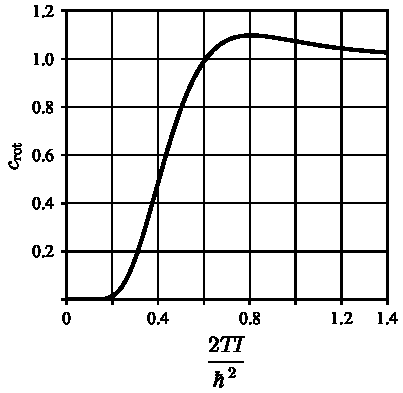
\includegraphics[width=7cm]{fig4.pdf}\\[0.3em]{\small 图 4}\end{minipage}\par\nopagebreak

\section{分子由相同原子构成的双原子气体.分子的转动}

由相同原子构成的双原子分子具有一些特点，有必要对前节中得到的某些公式加以修改.

首先来讨论使我们可以作经典考虑的高温极限情形，由于两个核是相同的，分子轴的两个相反的取向（区别只在于两个核的置换）现在对应于分子在物理上的同一个状态.因此经典的配分函数 (47.9) 应该除以2.这个情况也使得化学常数变为
\begin{equation}
  \zeta_{\mathrm{rot}}=\ln\frac{I}{\hbar^2};
\end{equation}
相当于在 $\zeta_{\mathrm{tr}}+\zeta_{\mathrm{rot}}$ 之和 (47.12) 中去掉了对数宗量中的因子2.

在需要作量子考虑的温度下会引起更重要的变化.由于整个问题的兴趣事实上只在于把它应用于氢的两种同位素（$\mathrm{H}_2$ 和 $\mathrm{D}_2$），下面我们就只注意这两种气体了.大家知道（参看第三卷§86），由于核的量子力学对称性的要求，使得在电子谱项 ${}^1\Sigma_g^{+}$（氢分子的基态谱项）中偶数 $K$ 值的和奇数 $K$ 值的转动能级具有不同的核简并度：偶数（奇数）$K$ 的能级只在两个核的自旋之和是偶数（奇数）的情形下出现，并且当核自旋 $i$ 为半整数时具有相对简并度：
\begin{equation*}
  g_g=\frac{i}{2i+1},\qquad g_u=\frac{i+1}{2i+1},
\end{equation*}
当 $i$ 为整数时具有相对简并度
\begin{equation*}
  g_g=\frac{i+1}{2i+1},\qquad g_u=\frac{i}{2i+1}.
\end{equation*}
按照通常采用的氢的术语，处于核统计权重较大的状态中的氢分子称为\textbf{正氢分子}，而处于核统计权重较小的状态中的氢分子称为\textbf{仲氢分子}.因此，分子 $\mathrm{H}_2$ 和 $\mathrm{D}_2$ 具有以下的统计权重值：
\begin{equation*}
  \mathrm{H}_2\Big(i=\frac{1}{2}\Big)\left\{
  \begin{aligned}
    &\text{正氢 }g_u=\frac{3}{4},\\
    &\text{仲氢 }g_g=\frac{1}{4},
  \end{aligned}\right.
  \qquad
  \mathrm{D}_2\left(i=1\right)\left\{
  \begin{aligned}
    &\text{正氢 }g_g=\frac{2}{3},\\
    &\text{仲氢 }g_u=\frac{1}{3}.
  \end{aligned}\right.
\end{equation*}
下标 $g$ 表示分子具有偶数的总核自旋（对于 $\mathrm{H}_2$ 是0，对于 $\mathrm{D}_2$ 是0或2）和偶数的转动角动量 $K$；下标 $u$ 表示奇数的总核自旋（对于 $\mathrm{H}_2$ 和 $\mathrm{D}_2$ 都是1）和奇数的 $K$ 值.

在具有不同原子的分子中，全部转动能级的核简并度都是相同的，因此假如考虑到这种简并性，那么也不过使得化学常数发生一个我们不感兴趣的改变，但在这里却导致配分函数本身形式的改变，现在应该把它写成如下的形式\footnote{我们采用归一化的核统计权重（即使得 $g_g+g_u=1$），这种归一化意味着：熵的计算是以 $\ln(2i+1)^2$ 的值为起点的，这相当于在§46末尾所采用的条件.}：
\begin{equation}
  Z_{\mathrm{rot}}=g_gZ_g+g_uZ_u,
\end{equation}
式中
\begin{equation}
\begin{aligned}
  Z_g&=\sum_{K=0,2,\cdots}\left(2K+1\right)
  \exp\Big[-\frac{\hbar^2}{2IT}K(K+1)\Big],\\
  Z_u&=\sum_{K=1,3,\cdots}\left(2K+1\right)
  \exp\Big[-\frac{\hbar^2}{2IT}K(K+1)\Big].
\end{aligned}
\end{equation}
自由能发生相应的改变：
\begin{equation}
  F_{\mathrm{rot}}=-NT\ln\left(g_gZ_g+g_uZ_u\right),
\end{equation}
其余的热力学量亦然.在高温下，
\begin{equation*}
  Z_g\approx Z_u\approx\frac{1}{2}Z_{\mathrm{rot}}=\frac{TI}{\hbar^2},
\end{equation*}
因此，对于自由能仍旧得到以前的经典表达式，这正是理所当然的.

当 $T\to0$ 时，和式 $Z_g$ 趋近于1，而 $Z_u$ 按指数规律趋近于0；所以，在低温下气体的行为就像单原子气体的情形一样（比热 $c_{\mathrm{rot}}=0$），对气体的化学常数只需要附加上一个“核部分”，它等于 $\zeta_{\mathrm{nuc}}=\ln g_g$.

显然，上述各公式只适合于处于完全热平衡状态的气体.在这样的气体中，正氢分子数和仲氢分子数的比值是温度的确定函数，按照玻尔兹曼分布它等于
\begin{equation}
  \left.
  \begin{aligned}
    \chi_{\mathrm{H}_2}&=\frac{N_{\text{正}\mathrm{H}_2}}{N_{\text{仲}\mathrm{H}_2}}
    =\frac{g_uZ_u}{g_gZ_g}=\frac{3Z_u}{Z_g},\\
    \frac{1}{\chi_{\mathrm{D}_2}}&=\frac{N_{\text{正}\mathrm{D}_2}}{N_{\text{仲}\mathrm{D}_2}}
    =\frac{g_gZ_g}{g_uZ_u}=\frac{2Z_g}{Z_u},
  \end{aligned}
  \right\}
\end{equation}
当温度从0变到 $\infty$ 时，比值 $\chi_{\mathrm{H}_2}$ 从0变到3，而 $\chi_{\mathrm{D}_2}$ 从0变到 $\dfrac{1}{2}$（当 $T=0$ 时，所有的分子当然都处于 $K$ 最小的状态，即处于 $K=0$ 的状态，这相当于纯仲 $\mathrm{H}_2$ 或纯正 $\mathrm{D}_2$）.

但是必须注意：在分子碰撞时，总核自旋改变的概率是非常小的.因此正氢分子和仲氢分子的行为实际上就像氢的两种彼此不能转变\footnote{不存在特殊的催化剂时.}的不同变体一样.因此在实际上碰到的并不是平衡的气体，而是正态和仲态的非平衡混合物，它们的相对的量是一个给定的常数值\footnote{对于通常长时间处于室温下的气体来讲，这个比值等于 $\chi_{\mathrm{H}_2}=3$，$\chi_{\mathrm{D}_2}=\dfrac{1}{2}$.}.这种混合物的自由能等于两种成分的自由能之和.

特别是，当 $\chi=\infty$（纯正 $\mathrm{H}_2$ 或纯仲 $\mathrm{D}_2$）时，我们有：
\begin{equation*}
  F_{\mathrm{tot}}=-NT\ln\left(g_uZ_u\right).
\end{equation*}
在低温下 $\Big(\dfrac{\hbar^2}{2IT}\gg1\Big)$，在 $Z_u$ 中可以只保留和式的第一项，因此有 $Z_u=3\exp\Big(-\dfrac{\hbar^2}{IT}\Big)$，因而自由能为
\begin{equation*}
  F_{\mathrm{rot}}=N\frac{\hbar^2}{I}-NT\ln\left(3g_u\right).
\end{equation*}
这表示：气体的行为就像单原子气体一样（$c_{\mathrm{rot}}=0$），并且在化学常数中出现一个附加项 $\ln3g_u$，而在能量中出现一个常数项 $\dfrac{N\hbar^2}{I}$，相当于全部分子都具有 $K=1$ 时的转动能.

\section{双原子气体.原子的振动}

气体热力学量的振动部分在非常高的温度下要比转动部分重要得多，因为谱项振动结构的间距比转动结构的间距大得多\footnote{举例来说，某些双原子气体的 $\dfrac{\hbar\omega}{k}$ 值为：$\mathrm{H}_2$ 6100K，$\mathrm{N}_2$ 3340K，$\mathrm{O}_2$ 2230K，NO 2690K，HCl 4140K.}.

但是，我们将认为温度只高到这样的程度：太高的振动能级基本上都没有被激发.这时振动是微小的（因而也是简谐的），因而能级由 (47.4) 中用过的通常的表达式 $\hbar\omega\big(v+\dfrac{1}{2}\big)$ 来决定.

振动配分函数 $Z_{\mathrm{vib}}$ (47.4) 的计算是很容易的.由于级数收敛得很快，可以在形式上把求和扩展到 $v=\infty$.我们假定以最低的（$v=0$）振动能级作为计算分子能量的起点（即把 $\dfrac{\hbar\omega}{2}$ 包括到 (47.1) 中的常数 $\varepsilon_0$ 中去）.

于是我们有：
\begin{equation*}
  Z_{\mathrm{vib}}=\sum_{v=0}^{\infty}\mathrm{e}^{-\frac{\hbar\omega}{T}v}
  =\frac{1}{1-\mathrm{e}^{-\frac{\hbar\omega}{T}}},
\end{equation*}
由此得出自由能为
\begin{equation}
  F_{\mathrm{vib}}=NT\ln\Big(1-\mathrm{e}^{-\frac{\hbar\omega}{T}}\Big),
\end{equation}
熵为
\begin{equation}
  S_{\mathrm{vib}}=-N\ln\Big(1-\mathrm{e}^{-\frac{\hbar\omega}{T}}\Big)
  +\frac{N\hbar\omega}{T\big(\mathrm{e}^{\frac{\hbar\omega}{T}}-1\big)},
\end{equation}
能量为
\begin{equation}
  E_{\mathrm{vib}}=\frac{N\hbar\omega}{\mathrm{e}^{\frac{\hbar\omega}{T}}-1}
\end{equation}
比热为
\begin{equation}
  c_{\mathrm{vib}}=\Big(\frac{\hbar\omega}{T}\Big)^{2}
  \frac{\mathrm{e}^{\frac{\hbar\omega}{T}}}
  {\big(\mathrm{e}^{\frac{\hbar\omega}{T}}-1\big)^{2}}.
\end{equation}
在图5中我们描出了 $c_{\mathrm{vib}}$ 与 $\dfrac{T}{\hbar\omega}$ 的函数关系曲线.

\par\nopagebreak\noindent\begin{minipage}{\linewidth}\centering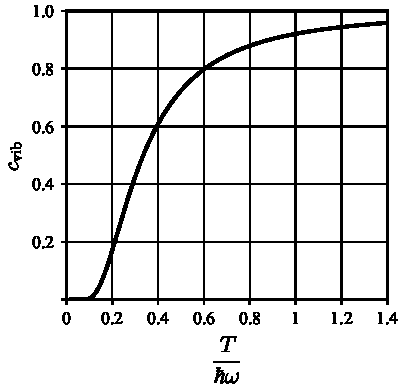
\includegraphics[width=7cm]{fig5.pdf}\\[0.3em]{\small 图 5}\end{minipage}\par\nopagebreak

在低温下（$\hbar\omega\gg T$），所有这些量都按指数规律趋于零：
\begin{equation}
\begin{aligned}
  F_{\mathrm{vib}}&=-NT\mathrm{e}^{-\frac{\hbar\omega}{T}},\\
  c_{\mathrm{vib}}&=\Big(\frac{\hbar\omega}{T}\Big)^{2}
  \mathrm{e}^{-\frac{\hbar\omega}{T}}.
\end{aligned}
\end{equation}
在高温下（$\hbar\omega\ll T$），我们有：
\begin{equation}
  F_{\mathrm{vib}}=-NT\ln T+NT\ln\hbar\omega-N\frac{\hbar\omega}{2},
\end{equation}
与此对应的常数比热为 $c_{\mathrm{vib}}=1$\footnote{再次与§44的经典结果一致.}，化学常数为 $\zeta_{\mathrm{vib}}=-\ln(\hbar\omega)$.把它们分别同 (47.11)，(47.12) 的值相加，我们求得在温度 $T\gg\hbar\omega$ 时双原子气体的总比热等于\footnote{从图5中可以看到，实际上 $c_{\mathrm{vib}}$ 在 $T\approx\hbar\omega$ 时已经趋近于它的极限值 1 了（例如，当 $\dfrac{T}{\hbar\omega}=1$ 时，$c_{\mathrm{vib}}=0.93$）.经典表达式可以适用的实用判别条件可以写为
\begin{equation*}
  T\gg\frac{\hbar\omega}{3}.
\end{equation*}}
\begin{equation}
  c_v=\frac{7}{2},\qquad c_p=\frac{9}{2},
\end{equation}
而化学常数为
\begin{equation}
  \zeta=\ln\Big[\frac{(2)I}{\omega\hbar^6}\Big(\frac{m}{2\pi}\Big)^{3/2}\Big].
\end{equation}
在这个公式中，对于由相同原子构成的分子来说，应该把因子 (2) 去掉.$E_{\mathrm{vib}}$ 的展开式中的前两项等于
\begin{equation}
  E_{\mathrm{vib}}=NT-\frac{1}{2}N\hbar\omega.
\end{equation}
式中出现的常数项 $-\dfrac{1}{2}N\hbar\omega$ 是因为我们计算能量是以最低的量子能级作为起点的（即从“零点振动”能开始算起），但是经典能量应该从势能的极小值开始算起.

当然，自由能的表达式 (49.6) 也可以用经典的方法求出来，因为当 $T\gg\hbar\omega$ 时，重要的是大的量子数 $v$，对于这些量子数来讲，运动是准经典的.角频率为 $\omega$ 的微振动的经典能量具有形式
\begin{equation*}
  \varepsilon_{\mathrm{vib}}(p,q)=\frac{p^2}{2m'}+\frac{m'\omega^2q^2}{2}
\end{equation*}
（$m'$ 是约化质量）.利用 $\varepsilon$ 的这个表达式来进行积分，就给出了配分函数的值
\begin{equation}
  Z_{\mathrm{vib}}=\frac{1}{2\pi\hbar}\iint
  \exp\Big(-\frac{\varepsilon_{\mathrm{vib}}}{T}\Big)\mathrm{d}p\,\mathrm{d}q
  =\frac{T}{\hbar\omega},
\end{equation}
它与 (49.6)\footnote{这个值是把对 $v$ 的求和用对 $\mathrm{d}v$ 的积分来代替后求得的.} 相对应（由于积分收敛很快，对 $\mathrm{d}q$ 的积分可以从积分限 $-\infty$ 积到 $+\infty$）.

在足够高的温度下，$v$ 值很大的振动也被激发，在这种温度下，振动的非简谐性的效应以及振动同分子转动的相互作用的效应都变得重要了（这两种效应原则上是同一数量级的）.由于 $v$ 很大，对热力学量的相应的修正可以用经典的方法来确定.

我们把分子看成由两个粒子所构成的力学系统，在相对于它们的质心为静止的坐标系中，它们按规律 $U(r)$ 相互作用着.经典地讲，以精确方式描述系统的转动和振动的能量（哈密顿函数）是动能（具有约化质量 $m'$ 的粒子的能量）和势能 $U(r)$ 之和.配分函数在对动量进行积分后归结为对坐标的积分：
\begin{equation*}
  \int\mathrm{e}^{-\frac{U(r)}{T}}\mathrm{d}V,
\end{equation*}
对角度（在球坐标中）进行积分后，剩下的积分为
\begin{equation*}
  \int_0^{\infty}\mathrm{e}^{-\frac{U(r)}{T}}r^2\,\mathrm{d}r.
\end{equation*}
如果令 $U(r)=U_0+\dfrac{1}{2}m'\omega^2(r-r_0)^2$，并且在积分时把变化缓慢的因子 $r^2$ 用 $r_0^2$ 来代替（其中 $r_0$ 是两个粒子间的平衡距离，而 $U_0=U(r_0)$），那么就可以获得相当于分子的转动和各种简谐振动都是独立的近似.为了考虑振动的非简谐性以及各种振动同转动的相互作用，我们现在把 $U(r)$ 写成
\begin{equation}
  U(r)=U_0+\frac{m'\omega^2r_0^2}{2}
  \left(\xi^2-\alpha\xi^3+\beta\xi^4\right)
\end{equation}
（$\xi=\dfrac{r}{r_0}-1$，$\alpha$ 和 $\beta$ 是常数\footnote{这两个常数可以用分子的光谱常数来表示（参看本教程第三卷§82）.}），然后从被积式中把因子
\begin{equation*}
  \exp\Bigg[-\frac{1}{T}\Big(U_0+\frac{1}{2}m'\omega^2r_0^2\xi^2\Big)\Bigg]
\end{equation*}
提出来，再把被积式按 $\xi$ 的幂次展开.在展开式中仅须保留在积分以后给出温度下一高次幂的那些项；对 $\mathrm{d}\xi$ 从积分限 $-\infty$ 积到 $+\infty$.展开式的零阶项就是配分函数的通常的值，而其余所有的项都是所求的修正项.我们把中间的计算省略掉，而直接把对自由能的修正的最后结果写出来：
\begin{equation}
  F_{\mathrm{anh}}=-NT^2\frac{1}{2I\omega^2}
  \Big(1+3\alpha-\frac{3}{2}\beta+\frac{15}{8}\alpha^2\Big).
\end{equation}
由此可见，由于振动的非简谐性（以及它们同转动的相互作用）在自由能中所引起的修正项与温度的平方成正比.相应地，对比热所附加的修正项与温度的一次方成正比.

\section{双原子气体.电子角动量的影响}

某些分子（当然，为数是不多的）在它们的电子基态中具有不等于零的轨道角动量或自旋.

大家知道，由于不等于零的轨道角动量 $\Lambda$ 的存在，电子谱项成为二重简并的，对应于轨道角动量相对于分子轴的两种可能的取向\footnote{严格地讲，谱项是分裂成两个能级的（称为 $\Lambda$-二重态），但是这两个能级之间的距离是如此的微小，以至在这里可以完全忽略不计.}.这种情况对气体的热力学量的影响是：由于配分函数增加了一倍，化学常数附加了一个量
\begin{equation}
  \zeta_{\Lambda}=\ln2.
\end{equation}
由于不等于零的自旋 $S$ 的存在，谱项分裂成 $2S+1$ 个谱项；但是（当 $\Lambda=0$ 时），这些精细结构的间距是如此的微小，以至在计算热力学量时总是可以忽略不计.自旋的存在仅仅导致所有的能级的简并度增加 $2S+1$ 倍，与此相应，化学常数附加了一个量
\begin{equation}
  \zeta_S=\ln\left(2S+1\right).
\end{equation}
出现在 $S\neq0$，$\Lambda\neq0$ 的精细结构需要特别的考虑.在这种情形下，精细结构的间距所可能达到的值使我们在计算热力学量时必须考虑到它们.我们来推导二重态电子谱项情形的公式.\footnote{这种情形在 NO 中出现；分子 NO 的基态电子谱项是二重态 $\Pi_{\frac{1}{2}\cdot\frac{3}{2}}$，其宽度（以 K 为单位）等于 $\Delta=178$K.二重态的两个组态都是二重简并的.\par
在氧中发生特殊的情况.分子 $\mathrm{O}_2$ 的基态电子谱项是距离非常窄的三重态 $^3\Sigma$，它们的宽度可以忽略不计.但是由于偶然的原因，下一个（激发态的）谱项 $^1\Delta$（二重简并的）相距不太远：$\Delta=11300$K，在高温时可以被激发，因而对热力学量会有影响.}电子二重态的每个组态都具有它自己的振动的和转动的结构，但参量可以认为是相同的.因此在配分函数 (47.2) 中还要出现一个因子：
\begin{equation*}
  Z_{\mathrm{el}}=g_0+g_1\mathrm{e}^{-\frac{\Delta}{T}},
\end{equation*}
式中 $g_0,g_1$ 是二重态的两个组态的简并度，$\Delta$ 是它们之间的距离.相应地，自由能附加了一项“电子的”部分：
\begin{equation}
  F_{\mathrm{el}}=-NT\ln\Big(g_0+g_1\mathrm{e}^{-\frac{\Delta}{T}}\Big).
\end{equation}
我们也可以写出“电子的”比热：
\begin{equation}
  c_{\mathrm{el}}=\frac{\Big(\dfrac{\Delta}{T}\Big)^{2}}
  {\Big[1+\dfrac{g_0}{g_1}\mathrm{e}^{\frac{\Delta}{T}}\Big]
  \Big[1+\dfrac{g_1}{g_0}\mathrm{e}^{-\frac{\Delta}{T}}\Big]},
\end{equation}
它应该添加到比热的其余部分上.在 $T\to0$ 和 $T\to\infty$ 这两种极限情形下，$c_{\mathrm{el}}$ 显然趋向于0，而在温度 $T\sim\Delta$ 时具有极大值.

\begin{xiti}

\noindent{\heiti 习题}\quad 试确定由 $\mathrm{O}_2$ 分子第一激发态电子谱项（参看 (50.2) 后的脚注）所引起的氧自由能修正项.温度比振动量子大得多，但是比基态谱项 $^3\Sigma$ 和激发态谱项 $^1\Delta$ 之间的距离 $\Delta$ 小得多.

解：配分函数为
\begin{equation*}
  Z=3\frac{T}{\hbar\omega}\cdot\frac{TI}{\hbar^2}
  +2\mathrm{e}^{-\frac{\Delta}{T}}\cdot\frac{T}{\hbar\omega'}
  \cdot\frac{TI'}{\hbar^2},
\end{equation*}
式中第一项和第二项各为基态谱项的和激发态谱项的配分函数，每一项都是电子因子、振动因子和转动因子的乘积.因此，所求的对自由能的修正项为
\begin{equation*}
  F_{1\Delta}=-NT\ln\Big(1+\frac{2\omega r_0'^2}{3\omega'r_0^2}
  \mathrm{e}^{-\frac{\Delta}{T}}\Big)
  \approx-NT\frac{2\omega r_0'^2}{3\omega'r_0^2}
  \mathrm{e}^{-\frac{\Delta}{T}},
\end{equation*}
式中 $\omega,r_0$ 和 $\omega',r_0'$ 各为在电子基态和电子激发态中的角频率和原子核之间的平衡距离.

\end{xiti}

\section{多原子气体}

如同双原子气体一样，多原子气体的自由能可以表示为三部分之和——平动的、转动的和振动的.平动部分仍旧由比热 $c_{\mathrm{tr}}$ 和化学常数 $\zeta_{\mathrm{tr}}$ 即
\begin{equation}
  c_{\mathrm{tr}}=\frac{3}{2},\qquad
  \zeta_{\mathrm{tr}}=\frac{3}{2}\ln\frac{m}{2\pi\hbar^2}
\end{equation}
来表征.

由于多原子分子的转动惯量值很大（因而相应地，转动量子很小），它们的转动总是可以经典地来考虑\footnote{转动的量子效应只有在甲烷 $\mathrm{CH}_4$ 中才会观察到，这种效应大约在 50K 的温度下出现（参看本节的习题）.}.多原子分子具有三个转动自由度，因而在一般情况下具有三个不同的主转动惯量 $I_1,I_2,I_3$；因此它的转动动能是
\begin{equation}
  \varepsilon_{\mathrm{rot}}=\frac{M_{\xi}^2}{2I_1}
  +\frac{M_{\eta}^2}{2I_2}+\frac{M_{\zeta}^2}{2I_3}
\end{equation}
式中 $\xi,\eta,\zeta$ 是转动坐标系的坐标，其坐标轴同分子的惯量主轴重合（我们暂时不考虑构成分子的诸原子排列在一条直线上的特殊情形）.这个表达式应该代入到配分函数
\begin{equation}
  Z_{\mathrm{rot}}=\int{}'\mathrm{e}^{-\frac{\varepsilon_{\mathrm{rot}}}{T}}\mathrm{d}\tau_{\mathrm{rot}},
\end{equation}
其中
\begin{equation*}
  \mathrm{d}\tau_{\mathrm{rot}}
  =\frac{1}{(2\pi\hbar)^3}\mathrm{d}M_{\xi}\mathrm{d}M_{\eta}\mathrm{d}M_{\zeta}
  \mathrm{d}\varphi_{\xi}\mathrm{d}\varphi_{\eta}\mathrm{d}\varphi_{\zeta},
\end{equation*}
像平常一样，积分号上的一撇表示：积分应该只对分子在物理上彼此不同的取向来进行.

如果分子具有某些对称轴，那么绕这些轴的某些转动使分子同它本身重合，因而其结果只不过是相同原子的置换.显然，分子在物理上相同的取向的数目等于分子绕各对称轴所容许的各种旋转（包括恒等变换——旋转360°——在内）的数目.用 $\sigma$ 来代表这个数目\footnote{例如，对于 $\mathrm{H}_2\mathrm{O}$（等腰三角形）来讲，$\sigma=2$；对于 $\mathrm{NH}_3$（正三角锥体）来讲，$\sigma=3$；对于 $\mathrm{CH}_4$（正四面体）来讲，$\sigma=12$；对于 $\mathrm{C}_6\mathrm{H}_6$（正六角形）来讲，$\sigma=12$.}，我们可以在 (51.3) 中直接对一切取向进行积分，再把整个表达式除以 $\sigma$.

在三个无限小转动角度的乘积 $\mathrm{d}\varphi_{\xi}\mathrm{d}\varphi_{\eta}\mathrm{d}\varphi_{\zeta}$ 中，可以把 $\mathrm{d}\varphi_{\xi}\mathrm{d}\varphi_{\eta}$ 看作是相对于 $\zeta$ 轴方向的立体角元 $\mathrm{d}o_{\zeta}$.对 $\mathrm{d}o_{\zeta}$ 的积分是与对 $\mathrm{d}\varphi_{\zeta}$（绕 $\zeta$ 轴本身的转动）的积分无关的，进行积分的结果等于 $4\pi$.以后对 $\mathrm{d}\varphi_{\zeta}$ 进行积分又给出 $2\pi$.再对 $\mathrm{d}M_{\xi}\mathrm{d}M_{\eta}\mathrm{d}M_{\zeta}$ 进行积分（积分限从 $-\infty$ 到 $+\infty$），结果我们求得：
\begin{equation*}
  Z_{\mathrm{rot}}=\frac{8\pi^2}{\sigma(2\pi\hbar)^3}(2\pi T)^{3/2}
  \left(I_1I_2I_3\right)^{1/2}
  =\frac{(2T)^{3/2}\left(\pi I_1I_2I_3\right)^{1/2}}{\sigma\hbar^3}.
\end{equation*}
由此得出自由能
\begin{equation}
  F_{\mathrm{rot}}=-\frac{3}{2}NT\ln T
  -NT\ln\frac{\left(8\pi I_1I_2I_3\right)^{1/2}}{\sigma\hbar^3}.
\end{equation}
因此按照§44，转动比热是：
\begin{equation}
  c_{\mathrm{rot}}=\frac{3}{2},
\end{equation}
而化学常数等于
\begin{equation}
  \zeta_{\mathrm{rot}}=\ln\frac{\left(8\pi I_1I_2I_3\right)^{1/2}}{\sigma\hbar^3}.
\end{equation}
如果多原子分子中所有的原子都排列在一条直线上（直线型分子），那么它也像双原子分子一样，具有两个转动自由度和一个转动惯量 $I$.转动比热和化学常数也像双原子气体一样，等于
\begin{equation}
  c_{\mathrm{rot}}=1,\qquad
  \zeta_{\mathrm{rot}}=\ln\frac{2I}{\sigma\hbar^2},
\end{equation}
在这里对于非对称的分子（例如，NNO）来讲，$\sigma=1$，对于中心对称的分子（例如，OCO）来讲，$\sigma=2$.

对多原子气体自由能的振动部分的计算类似于我们对双原子气体所作的计算.区别在于：多原子气体所具有的振动自由度不止一个，而是若干个.就是说，$n$ 个原子的（非直线型）分子显然具有 $r_{\mathrm{vib}}=3n-6$ 个振动自由度；而对于直线型的 $n$ 个原子的分子，$r_{\mathrm{vib}}=3n-5$（参看§44）.振动自由度的数目决定分子的所谓简正振动的数目，每一种简正振动有它自己的角频率 $\omega_{\alpha}$（角标 $\alpha$ 是简正振动的编号）.必须注意：这些 $\omega_{\alpha}$ 中的某些频率可能彼此相同；在这种情形下我们说角频率是简并的.

在简谐近似下，我们认为振动很微小（我们所考虑的也只是这样的温度），这时所有的简正振动都是独立的，因而振动能量就是各个振动的能量之和.因此振动配分函数分解成各个振动的配分函数之积，而所得到的自由能 $F_{\mathrm{vib}}$ 是 (49.1) 型的表达式之和
\begin{equation}
  F_{\mathrm{vib}}=NT\sum_{\alpha}\ln\Big(1-\mathrm{e}^{-\frac{\hbar\omega_{\alpha}}{T}}\Big).
\end{equation}
在这个和式中每一个角频率出现的次数等于它的简并度.对于其它热力学量的振动部分也相应地得到这种类型的和式.

每一种简正振动在各自的经典情形（$T\gg\hbar\omega_{\alpha}$）下对比热的贡献等于 $c_{\mathrm{vib}}^{(\alpha)}$；当 $T$ 比最大的一个 $\hbar\omega_{\alpha}$ 还大时，我们就会得到
\begin{equation}
  c_{\mathrm{vib}}=r_{\mathrm{vib}}.
\end{equation}
但是，事实上这个极限是达不到的，因为多原子分子通常在比这低得多的温度下就已经分解了.

多原子分子的各种角频率 $\omega_{\alpha}$ 的值通常是散布在一个很大的范围内的.随着温度的升高，各种简正振动逐个“计入”到比热中去.这种情况使得多原子气体的比热往往可以在相当宽阔的温度范围内认为几乎是常数.

我们现在来讨论一种从振动到转动的特殊转变的可能性，乙烷分子 $\mathrm{C}_2\mathrm{H}_6$ 就是这种例子.这种分子由两个 $\mathrm{CH}_3$ 原子团构成，它们彼此相隔一定的距离，并且以一定的方式相对地取向.分子的简正振动之一是“扭转振动”，在这种振动下，一个 $\mathrm{CH}_3$ 原子团相对于另一个 $\mathrm{CH}_3$ 扭转.随着振动能量的增加，它们的振幅也在增长，最后在足够高的温度下，振动转变为自由转动.结果这个自由度对比热的贡献在振动被完全激发时大约达到1，当温度继续增高时开始下降，渐近地趋近于转动的特征值1/2.

最后，应当指出：如果分子具有不等于零的自旋 $S$（例如，分子 $\mathrm{NO}_2$，$\mathrm{ClO}_2$），那么就使得化学常数附加一个量
\begin{equation}
  \zeta_S=\ln\left(2S+1\right).
\end{equation}

\begin{xiti}

\noindent{\heiti 习题}\quad 试确定甲烷在低温下的转动配分函数.

解：在本节第一个脚注中已经指出，在足够低的温度下，甲烷的 $Z_{\mathrm{rot}}$ 应该用量子方法计算.

$\mathrm{CH}_4$ 分子具有正四面体的形状，因而转动时像一个球状陀螺，因此它的转动能级等于 $\dfrac{\hbar^2}{2I}J(J+1)$，其中 $I$ 是三个主转动惯量的共同值，$J$ 是转动量子数.因为 H 核的自旋等于 $i=\dfrac{1}{2}$，而碳原子 $\mathrm{C}^{12}$ 的核自旋等于零，所以 $\mathrm{CH}_4$ 分子的总核自旋可以等于0,1,2（相应的核统计权重为1,3,5）\footnote{参看本教程第三卷§105 习题5.}.对于每一个给定的 $J$ 值来讲，对应于总核自旋每一个不同的值存在着一定数目的状态.在下表中给出了前五个 $J$ 值在不同总核自旋时的状态数：

\begin{center}
\begin{tabular}{lccc}
核自旋： & 0 & 1 & 2 \\
$J=0$ & — & — & 1 \\
$J=1$ & — & 1 & — \\
$J=2$ & 2 & 1 & — \\
$J=3$ & — & 2 & 1 \\
$J=4$ & 2 & 2 & 1
\end{tabular}
\end{center}

如果我们假定熵是以 $\ln(2i+1)^4=\ln16$ 的值作为起点来计算的（参看§48第一个脚注），那么在考虑到转动角动量和核自旋各种取向的总简并度后所得到的配分函数 $Z_{\mathrm{rot}}$ 的值还必须除以16.结果我们得到：
\begin{equation*}
  Z_{\mathrm{rot}}=\frac{5}{16}+\frac{9}{16}\mathrm{e}^{-\frac{\hbar^2}{IT}}
  +\frac{25}{16}\mathrm{e}^{-3\frac{\hbar^2}{IT}}
  +\frac{77}{16}\mathrm{e}^{-6\frac{\hbar^2}{IT}}
  +\frac{117}{16}\mathrm{e}^{-10\frac{\hbar^2}{IT}}+\cdots.
\end{equation*}

\end{xiti}

\section{气体的磁性}

置于外磁场 $\boldsymbol{H}$ 中的物体还需要一个宏观量来表征——物体在场中所具有的磁矩 $\mathfrak{M}$.对于理想气体，该磁矩 $\mathfrak{M}=N\bar{\boldsymbol{m}}$（式中 $\bar{\boldsymbol{m}}$ 是原子或分子的单粒子磁矩），因此，计算它只需要考虑气体的单个粒子在磁场中的行为.我们还要着重指出，因为作为稀薄介质的气体其磁化强度及密度都很小，所以可以忽略介质对磁场的影响，即认为作用在每个粒子上的磁场就是外磁场 $\boldsymbol{H}$.

当外磁场有微小变化 $\delta\boldsymbol{H}$ 时，气体的哈密顿量的变化是 $\delta\hat{H}=-\hat{\mathfrak{M}}\cdot\delta\boldsymbol{H}$，式中 $\hat{\mathfrak{M}}$ 是气体的磁矩算符\footnote{在经典力学中，磁场变化 $\delta\boldsymbol{H}$ 时粒子系统拉格朗日量的微小变化为 $\delta L=\mathfrak{M}(q,\dot{q})\cdot\delta\boldsymbol{H}$，式中 $\mathfrak{M}(q,\dot{q})$ 是系统的磁矩，为其动力学变量坐标与速度的函数（参看本教程第二卷，(45.3)）.哈密顿量的变化（在给定的坐标 $q$ 与动量 $p$ 下）与 $\delta L$ 的区别仅在于符号（参看第一卷，(40.7)）；$\delta H=-\mathfrak{M}(p,q)\cdot\delta\boldsymbol{H}$.在量子力学中哈密顿量的变化也有类似的表达式，并且 $\hat{\mathfrak{M}}$ 是磁矩算符，通过粒子的坐标与动量（以及它们的自旋）算符来表示.}.根据公式 (15.11)（另见 (11.4)），那里的外参量 $\lambda$ 现在应取作场 $\boldsymbol{H}$，因此我们有
\begin{equation}
  \mathfrak{M}=-\Big(\frac{\partial F}{\partial H}\Big)_{T,V,N}.
\end{equation}
为计算粒子在磁场中的自由能必须预先确定与场有关的气体粒子能级修正，我们先考虑单原子气体.原子在磁场中的哈密顿算符为
\begin{equation}
  \hat{H}=\hat{H}_0-\hat{\boldsymbol{m}}\cdot\boldsymbol{H}
  +\frac{e^2}{8mc^2}\sum_a\left(\boldsymbol{H}\times\boldsymbol{r}_a\right)^2,
\end{equation}
式中 $\hat{H}_0$ 是没有外场时原子的哈密顿算符，$e$ 和 $m$ 是电子的电荷与质量，$\boldsymbol{r}_a$ 是电子的坐标（求和对所有的电子进行），$\hat{\boldsymbol{m}}=-\beta\left(2\hat{\boldsymbol{S}}+\hat{\boldsymbol{L}}\right)$ 是原子的“内禀”磁矩算符（$\hat{\boldsymbol{S}}$ 和 $\hat{\boldsymbol{L}}$ 是电子的自旋和轨道角动量算符，$\beta=\dfrac{|e|\hbar}{2mc}$ 是玻尔磁子（参看第三卷§113）.把 (52.2) 中的第二项和第三项看成对 $\hat{H}_0$ 的微扰，我们确定精确到场的二阶的能级修正项，其形为
\begin{equation}
  \Delta\varepsilon_k\equiv\varepsilon_k-\varepsilon_k^{(0)}
  =-A_kH-\frac{1}{2}B_kH^2,
\end{equation}
其中
\begin{equation}
  A_k=\left(m_z\right)_{kk},
\end{equation}
\begin{equation}
  B_k=2\sum_{k'}{}'
  \frac{\left|\left(m_z\right)_{kk'}\right|^2}
  {\varepsilon_{k'}^{(0)}-\varepsilon_k^{(0)}}
  -\frac{e^2}{4mc^2}\sum_a\left(x_a^2+y_a^2\right)_{kk},
\end{equation}
这里 $z$ 轴沿 $\boldsymbol{H}$ 的方向；(52.5) 中的第一项来自 (52.2) 中 $\boldsymbol{H}$ 线性项的二阶微扰，而第二项来自哈密顿算符二次项的一阶微扰.

在计算自由能时，我们假设气体的温度不太低，从而修正项 $\Delta\varepsilon_k\ll T$.这时配分函数可按 $H$ 的幂次展开.精确到 $H$ 的平方项我们有
\begin{equation*}
  Z\equiv\sum_k\mathrm{e}^{-\frac{\varepsilon_k}{T}}
  =\sum_k\mathrm{e}^{-\frac{\varepsilon_k}{T}}
  \Big[1+\frac{A_kH}{T}+\frac{A_k^2H^2}{2T^2}+\frac{B_kH^2}{2T}\Big].
\end{equation*}
对 $k$ 的求和特别包含了对原子内禀磁矩 $\boldsymbol{m}$ 取向的平均（未微扰能级与磁矩无关）；考虑到对称性，显然，这时平均值 $\bar{A}$ 为零，于是有
\begin{equation*}
  Z=\Big[1+\frac{H^2}{2T}\Big(\frac{\overline{A^2}}{T}+\overline{B}\Big)\Big]
  \sum_k\mathrm{e}^{-\frac{\varepsilon_k}{T}},
\end{equation*}
式中横线表示按（无微扰场）玻尔兹曼分布求平均.把这个表达式代入 (41.4) 并随后求自由能对 $\boldsymbol{H}$ 的导数，就得到磁矩形如 $\mathfrak{M}=N\chi\boldsymbol{H}$，式中
\begin{equation}
  \chi=\frac{1}{T}\overline{A^2}+\overline{B}
\end{equation}
是气体的分子磁化率（J.~H.~Van Vleck, 1927）.我们考虑几种特殊情形.

我们考虑同基态能级与激发态能级中最接近能级（包括基态谱项的精细结构组态）之间的间距相比温度 $T$ 很小的情况.这时可以认为只有原子的基态（$k=0$）对平均值 $\overline{A^2}$ 与 $\overline{B}$ 有贡献.

如果原子（在基态中）既无自旋又无轨道角动量，在这种最简单的情况下，原子的内禀磁矩的所有矩阵元也等于0.这时 $A_0=0$，而只有第二项 $B_0$ 不等于零.由于 $L=S=0$ 态的波函数有球对称性，对角矩阵元（即对原子态的平均值）为 $\left(x_a^2\right)_{00}=\left(y_a^2\right)_{00}=\dfrac{1}{3}\left(r_a^2\right)_{00}$.结果我们求得
\begin{equation}
  \chi=-\frac{e^2}{6mc^2}\sum_a\left(r_a^2\right)_{00},
\end{equation}
即气体是抗磁的，具有与温度无关的磁化率（P.~朗之万，1905）\footnote{我们着重指出，这种抗磁性（在第三卷§113就已经指出）具有量子本性：虽然在(52.7)中不显含量子常数 $\hbar$，事实上它决定原子的“大小”.在这一方面我们指出，在经典统计学中物质的宏观磁性完全不出现.实际上，在经典力学中，磁场中系统的哈密顿量与没有磁场时的区别只在于用差 $\boldsymbol{P}-\dfrac{e}{c}\boldsymbol{A}(\boldsymbol{r})$ 代替粒子的动量 $\boldsymbol{p}$，这里 $\boldsymbol{P}$ 是广义动量，而 $\boldsymbol{A}(\boldsymbol{r})$ 是场的矢势.在配分函数中积分是对所有的动量 $\boldsymbol{P}$（以及坐标 $\boldsymbol{r}$）进行的.变量代换以后（从对 $\boldsymbol{P}$ 积分变到对 $\boldsymbol{p}=\boldsymbol{P}-\dfrac{e}{c}\boldsymbol{A}$ 积分），我们发现磁场通常从配分函数中因而也从所有热力学量中消失.}.

如果原子的内禀磁矩不为零，则 $A_0\neq0$ 且 (52.6) 中的第一项（在关于温度所作的假设下）比第二项大.根据定义 (52.4)，计算给出
\begin{equation*}
  A_0=-\beta gM_J,\qquad
  g=1+\frac{J(J+1)-L(L+1)+S(S+1)}{2J(J+1)},
\end{equation*}
式中 $g$ 为朗德因子，$M_J$ 是原子总角动量的投影（参看第三卷§113节）.(52.6) 中的求平均化为对 $M_J$ 求平均.注意到
\begin{equation*}
  \overline{M_J^2}=\frac{1}{2J+1}\sum_{M_J=-J}^{J}M_J^2
  =\frac{1}{3}J(J+1),
\end{equation*}
得
\begin{equation}
  \chi=\frac{\beta^2g^2}{3T}J(J+1).
\end{equation}
因此，气体是顺磁的，其磁化率遵从居里定律，与温度成反比（P.~朗之万，1905）\footnote{公式(52.8)不仅适用于气体，而且也适用于凝聚体，只要原子磁矩由于某种原因可以当成是“自由的”.例如稀土元素的固体盐类与溶液中的磁性就属于这种情况.这些离子的顺磁性与未被占满的 4f 壳层有关.这些较深层电子被外层电子所屏蔽而不受近邻原子影响，结果在磁性方面，这些离子就像稀薄气体的原子一样.}.

如果原子的轨道角动量和自旋都不等于零但数值相同（$L=S\neq0$），而且合成总角动量 $J=0$，那么内禀磁矩的对角矩阵元等于零，然而非对角矩阵元（对于多重态内的 $L,S,J\to L,S,J\pm1$ 跃迁）不为零.这时，$A_0=0$，而 (52.5) 的 $B_0$ 中第二项（抗磁性项）比第一项小，后者的分母含有相对较小的基态精细结构间距.这里 $B_0>0$：相对于基态能级，$k'$ 求和中的每一项无论分子还是分母都是正的.因此，在这种情况下气体是顺磁的，其磁化率与温度无关：$\chi=B_0$（J.~H.~Van Vleck, 1928）\footnote{这种情况可出现在铕盐的铕离子 $\mathrm{Eu}^{+++}$ 中（参看上注）.}.

分子气体的磁化率可用类似的方法计算.在通常温度下分子的转动是经典的.因此计算磁矩的矩阵元可以先对固定不动的原子核计算，然后再将分子看成如同是刚性的经典磁偶极子对分子的取向求平均（参看习题）\footnote{核运动所产生的磁矩与电子运动所产生的磁矩相比很小，因此总可以忽略不计.}.

\begin{xiti}

\noindent{\heiti 习题1}\quad 在 $T$ 同原子基态精细结构间距相比很小的情况下，确定单原子气体的磁化率.

解：在这种情况下，(52.6) 中的平均应该对原子多重态的所有组态求，并且所有组态的玻尔兹曼因子 $\big(\mathrm{e}^{-\frac{\varepsilon_k'}{T}}\big)$ 可以认为是相同的.这时，
\begin{equation*}
  \overline{A^2}=\overline{\left|\left\langle JM_J\middle|m_z\middle|JM_J\right\rangle\right|^2},
\end{equation*}
式中求平均对所有的值 $J$ 和 $M_J$（在给定的 $S$ 和 $L$ 下）进行.但是这种求平均的结果，与求平均在角动量 $S$ 和 $L$ 相加成 $J$ 之后还是之前没有关系；换句话说，可以对 $M_L$ 和 $M_S$ 独立求平均来计算
\begin{equation*}
  \overline{A^2}=\overline{\left|\left\langle M_LM_S\middle|m_z\middle|M_LM_S\right\rangle\right|^2},
\end{equation*}
注意到
\begin{equation*}
  \overline{M_SM_L}=\overline{M_S}\,\overline{M_L}=0,\qquad
  \overline{M_S^2}=\frac{1}{3}S(S+1),\qquad
  \overline{M_L^2}=\frac{1}{3}L(L+1),
\end{equation*}
得
\begin{equation*}
  \overline{A^2}=\beta^2\left[4S(S+1)+L(L+1)\right].
\end{equation*}
在 $\overline{B}$ 的 (52.5) 式中第二项可以忽略；第一项（由于它的分母即多重态间距很小而可能很大）在对多重态的组态求平均后变为零：在和式
\begin{equation*}
  \sum{}'\frac{\left|\left\langle JM_J\middle|m_z\middle|J'M_J'\right\rangle\right|^2}
  {\varepsilon_{J'}^{(0)}-\varepsilon_J^{(0)}}
\end{equation*}
中的求和，现在遍及所有的数 $J,J',M_J,M_J'$，而 $J$ 和 $J'$ 的互换的不同项相消.因此，磁化率为
\begin{equation*}
  \chi=\frac{\beta^2}{3T}\left[4S(S+1)+L(L+1)\right].
\end{equation*}

\noindent{\heiti 习题2}\quad 在与 $T$ 相比分子的电子基态精细结构间距很大时\footnote{在通常温度下，多重态的间距与转动能级结构间距相比明显地大，因而分子项属于 $a$ 型耦合（参看第三卷§83）.}，求双原子气体的磁化率.

解：在这种情况下，只要研究分子的基态能级即基态多重态的最低的组态就够了.在轨道角动量与自旋在分子轴上的投影为 $\Lambda$ 和 $\Sigma$ 的态中，分子磁矩的平均值为
\begin{equation*}
  \left\langle\Lambda\Sigma\middle|\boldsymbol{m}\middle|\Lambda\Sigma\right\rangle
  =-\beta\boldsymbol{n}\left(\Lambda+2\Sigma\right),
\end{equation*}
式中 $\boldsymbol{n}$ 是沿分子轴的单位矢量.在经典转动的情况下 $\overline{n_z^2}=\dfrac{1}{3}$，我们求得磁化率为
\begin{equation*}
  \chi=\frac{\beta^2}{3T}\left(\Lambda+2\Sigma\right)^2.
\end{equation*}

\noindent{\heiti 习题3}\quad 如果与 $T$ 相比精细结构间距很小（分子项属于 b 型），求上题.

解：在这种情况下，应该对多重态的所有组态求平均.在给定 $\Lambda$ 和自旋 $z$ 分量 $M_S$ 时，磁矩 $z$ 分量的对角矩阵元为
\begin{equation*}
  \left\langle\Lambda M_S\middle|m_z\middle|\Lambda M_S\right\rangle
  =-\beta\left(n_z\Lambda+2M_S\right).
\end{equation*}
把它的平方对 $M_S$ 的值和方向 $\boldsymbol{n}$ 求平均，就得到磁化率
\begin{equation*}
  \chi=\frac{\beta^2}{3T}\left[\Lambda^2+4S(S+1)\right].
\end{equation*}

\noindent{\heiti 习题4}\quad 确定 NO 气体的磁化率.分子的基态电子项为 $^2\Pi$（即 $\Lambda=1$，$S=\dfrac{1}{2}$），并且二重态的组态间距 $\Delta$ 与温度相当\footnote{它为 $\Delta=180$K.二重态的下态对应于自旋的轴分量 $\Sigma=-\dfrac{1}{2}$，而上态对应于 $\Sigma=\dfrac{1}{2}$.耦合项属于 $a$ 型.}.（J.~H.~Van Vleck, 1928）.

解：这里，在求 (52.6) 中的平均时必须考虑双能级的两个组态具有不同的玻尔兹曼因子.两种状态 $\left|\Lambda\Sigma\right\rangle$ 的磁矩对角矩阵元为
\begin{equation*}
  \left\langle 1,-\frac{1}{2}\middle|\boldsymbol{L}+2\boldsymbol{S}\middle|1,-\frac{1}{2}\right\rangle
  =\boldsymbol{n}-2\cdot\frac{1}{2}\boldsymbol{n}=\boldsymbol{0},
\end{equation*}
\begin{equation*}
  \left\langle 1,\frac{1}{2}\middle|\boldsymbol{L}+2\boldsymbol{S}\middle|1,\frac{1}{2}\right\rangle
  =2\boldsymbol{n},
\end{equation*}
由此得
\begin{equation*}
  \overline{A^2}=\frac{4}{3}\beta^2
  \frac{\mathrm{e}^{-\frac{\Delta}{T}}}{1+\mathrm{e}^{-\frac{\Delta}{T}}}.
\end{equation*}
对于这两种状态之间的跃迁，算符 $\hat{\boldsymbol{L}}$ 没有矩阵元（因为跃迁时 $\Sigma$ 改变而 $\Lambda$ 不变）.算符 $2S_z$ 的非对角矩阵元为
\begin{equation*}
  \left\langle 1,\frac{1}{2}\middle|2S_z\middle|1,-\frac{1}{2}\right\rangle
  =\left\langle 1,-\frac{1}{2}\middle|2S_z\middle|1,\frac{1}{2}\right\rangle
  =-1\cdot\sin\theta,
\end{equation*}
式中 $\theta$ 是 $\boldsymbol{n}$ 与 $z$ 轴间的夹角\footnote{算符 $S=\dfrac{\sigma}{2}$，式中 $\sigma$ 是量子化方向沿分子轴的泡利矩阵（也就是说，如果 $\xi\eta\zeta$ 是坐标轴且 $\zeta$ 轴沿 $\boldsymbol{n}$，则
$\sigma_\zeta=\begin{pmatrix}1&0\\0&-1\end{pmatrix}$）.}.根据 (52.5)（这里再次忽略第二项），有
\begin{equation*}
  \overline{B}=\frac{2\beta^2}{\Delta}\cdot\frac{2}{3}
  \frac{1-\mathrm{e}^{-\frac{\Delta}{T}}}{1+\mathrm{e}^{-\frac{\Delta}{T}}}
\end{equation*}
（因子 $\dfrac{2}{3}$ 来自 $\sin^2\theta$ 的平均）.磁化率的完全表达式可得如下式
\begin{equation*}
  \chi=\frac{\beta^2}{3T}f\Big(\frac{\Delta}{T}\Big),\qquad
  f(x)=\frac{4\left[1-\mathrm{e}^{-x}(1-x)\right]}{x\left(1+\mathrm{e}^{-x}\right)}.
\end{equation*}

\end{xiti}
